%%% Hlavní soubor. Zde se definují základní parametry a odkazuje se na ostatní části. %%%

%% Verze pro jednostranný tisk:
% Okraje: levý 40mm, pravý 25mm, horní a dolní 25mm
% (ale pozor, LaTeX si sám přidává 1in)
\documentclass[12pt,a4paper]{report}
\setlength\textwidth{145mm}
\setlength\textheight{247mm}
\setlength\oddsidemargin{15mm}
\setlength\evensidemargin{15mm}
\setlength\topmargin{0mm}
\setlength\headsep{0mm}
\setlength\headheight{0mm}
% \openright zařídí, aby následující text začínal na pravé straně knihy
\let\openright=\clearpage

\setcounter{secnumdepth}{3}

%% Pokud tiskneme oboustranně:
% \documentclass[12pt,a4paper,twoside,openright]{report}
% \setlength\textwidth{145mm}
% \setlength\textheight{247mm}
% \setlength\oddsidemargin{14.2mm}
% \setlength\evensidemargin{0mm}
% \setlength\topmargin{0mm}
% \setlength\headsep{0mm}
% \setlength\headheight{0mm}
% \let\openright=\cleardoublepage

%% Vytváříme PDF/A-2u
\usepackage[a-2u]{pdfx}

%% Přepneme na českou sazbu a fonty Latin Modern
\usepackage[czech]{babel}
\usepackage{lmodern}
\usepackage[T1]{fontenc}
\usepackage{textcomp}

%% Použité kódování znaků: obvykle latin2, cp1250 nebo utf8:
\usepackage[utf8]{inputenc}

%%% Další užitečné balíčky (jsou součástí běžných distribucí LaTeXu)
\usepackage{amsmath}        % rozšíření pro sazbu matematiky
\usepackage{amsfonts}       % matematické fonty
\usepackage{amsthm}         % sazba vět, definic apod.
\usepackage{bbding}         % balíček s nejrůznějšími symboly
			    % (čtverečky, hvězdičky, tužtičky, nůžtičky, ...)
\usepackage{bm}             % tučné symboly (příkaz \bm)
\usepackage{graphicx}       % vkládání obrázků
\usepackage{fancyvrb}       % vylepšené prostředí pro strojové písmo
\usepackage{indentfirst}    % zavede odsazení 1. odstavce kapitoly
\usepackage{natbib}         % zajištuje možnost odkazovat na literaturu
			    % stylem AUTOR (ROK), resp. AUTOR [ČÍSLO]
\usepackage[nottoc]{tocbibind} % zajistí přidání seznamu literatury,
                            % obrázků a tabulek do obsahu
\usepackage{icomma}         % inteligetní čárka v matematickém módu
\usepackage{dcolumn}        % lepší zarovnání sloupců v tabulkách
\usepackage{booktabs}       % lepší vodorovné linky v tabulkách
\usepackage{paralist}       % lepší enumerate a itemize
\usepackage{xcolor}         % barevná sazba

%%% Údaje o práci

% Název práce v jazyce práce (přesně podle zadání)
\def\NazevPrace{Evoluce robotů v simulovaném fyzikálním prostředí}

% Název práce v angličtině
\def\NazevPraceEN{Evolution of robots in a simulated physical environment}

% Jméno autora
\def\AutorPrace{Marek Bečvář}

% Rok odevzdání
\def\RokOdevzdani{2023}

% Název katedry nebo ústavu, kde byla práce oficiálně zadána
% (dle Organizační struktury MFF UK, případně plný název pracoviště mimo MFF)
\def\Katedra{Katedra softwaru a výuky informatiky}
\def\KatedraEN{Department of software and computer science education}

% Jedná se o katedru (department) nebo o ústav (institute)?
\def\TypPracoviste{Katedra}
\def\TypPracovisteEN{Department}

% Vedoucí práce: Jméno a příjmení s~tituly
\def\Vedouci{RNDr. František Mráz, CSc.}

% Pracoviště vedoucího (opět dle Organizační struktury MFF)
\def\KatedraVedouciho{Katedra softwaru a výuky informatiky}
\def\KatedraVedoucihoEN{Department of software and computer science education}

% Studijní program a obor
\def\StudijniProgram{Informatika}
\def\StudijniObor{Informatika se specializací Umělá inteligence}

% Nepovinné poděkování (vedoucímu práce, konzultantovi, tomu, kdo
% zapůjčil software, literaturu apod.)
\def\Podekovani{%
Poděkování.
}

% Abstrakt (doporučený rozsah cca 80-200 slov; nejedná se o zadání práce)
\def\Abstrakt{%
Abstrakt.
}
\def\AbstraktEN{%
Abstract.
}

% 3 až 5 klíčových slov (doporučeno), každé uzavřeno ve složených závorkách
\def\KlicovaSlova{%
{klíčová} {slova}
}
\def\KlicovaSlovaEN{%
{key} {words}
}

%% Balíček hyperref, kterým jdou vyrábět klikací odkazy v PDF,
%% ale hlavně ho používáme k uložení metadat do PDF (včetně obsahu).
%% Většinu nastavítek přednastaví balíček pdfx.
\hypersetup{unicode}
\hypersetup{breaklinks=true}

%% Definice různých užitečných maker (viz popis uvnitř souboru)
%%% Tento soubor obsahuje definice různých užitečných maker a prostředí %%%
%%% Další makra připisujte sem, ať nepřekáží v ostatních souborech.     %%%

%%% Drobné úpravy stylu

% Tato makra přesvědčují mírně ošklivým trikem LaTeX, aby hlavičky kapitol
% sázel příčetněji a nevynechával nad nimi spoustu místa. Směle ignorujte.
\makeatletter
\def\@makechapterhead#1{
  {\parindent \z@ \raggedright \normalfont
   \Huge\bfseries \thechapter. #1
   \par\nobreak
   \vskip 20\p@
}}
\def\@makeschapterhead#1{
  {\parindent \z@ \raggedright \normalfont
   \Huge\bfseries #1
   \par\nobreak
   \vskip 20\p@
}}
\makeatother

% Toto makro definuje kapitolu, která není očíslovaná, ale je uvedena v obsahu.
\def\chapwithtoc#1{
\chapter*{#1}
\addcontentsline{toc}{chapter}{#1}
}

% Trochu volnější nastavení dělení slov, než je default.
\lefthyphenmin=2
\righthyphenmin=2

% Zapne černé "slimáky" na koncích řádků, které přetekly, abychom si
% jich lépe všimli.
\overfullrule=1mm

%%% Makra pro definice, věty, tvrzení, příklady, ... (vyžaduje baliček amsthm)

\theoremstyle{plain}
\newtheorem{veta}{Věta}
\newtheorem{lemma}[veta]{Lemma}
\newtheorem{tvrz}[veta]{Tvrzení}

\theoremstyle{plain}
\newtheorem{definice}{Definice}

\theoremstyle{remark}
\newtheorem*{dusl}{Důsledek}
\newtheorem*{pozn}{Poznámka}
\newtheorem*{prikl}{Příklad}

%%% Prostředí pro důkazy

\newenvironment{dukaz}{
  \par\medskip\noindent
  \textit{Důkaz}.
}{
\newline
\rightline{$\qedsymbol$}
}

%%% Prostředí pro sazbu kódu, případně vstupu/výstupu počítačových
%%% programů. (Vyžaduje balíček fancyvrb -- fancy verbatim.)

\DefineVerbatimEnvironment{code}{Verbatim}{fontsize=\small, frame=single}

%%% Prostor reálných, resp. přirozených čísel
\newcommand{\R}{\mathbb{R}}
\newcommand{\N}{\mathbb{N}}

%%% Užitečné operátory pro statistiku a pravděpodobnost
\DeclareMathOperator{\pr}{\textsf{P}}
\DeclareMathOperator{\E}{\textsf{E}\,}
\DeclareMathOperator{\var}{\textrm{var}}
\DeclareMathOperator{\sd}{\textrm{sd}}

%%% Příkaz pro transpozici vektoru/matice
\newcommand{\T}[1]{#1^\top}

%%% Vychytávky pro matematiku
\newcommand{\goto}{\rightarrow}
\newcommand{\gotop}{\stackrel{P}{\longrightarrow}}
\newcommand{\maon}[1]{o(n^{#1})}
\newcommand{\abs}[1]{\left|{#1}\right|}
\newcommand{\dint}{\int_0^\tau\!\!\int_0^\tau}
\newcommand{\isqr}[1]{\frac{1}{\sqrt{#1}}}

%%% Vychytávky pro tabulky
\newcommand{\pulrad}[1]{\raisebox{1.5ex}[0pt]{#1}}
\newcommand{\mc}[1]{\multicolumn{1}{c}{#1}}


%% Titulní strana a různé povinné informační strany
\begin{document}
%%% Titulní strana práce a další povinné informační strany

%%% Titulní strana práce

\pagestyle{empty}
\hypersetup{pageanchor=false}

\begin{center}

\centerline{\mbox{
\includegraphics[width=166mm]{../img/logo-cs.pdf}}}

\vspace{-8mm}
\vfill

{\bf\Large BAKALÁŘSKÁ PRÁCE}

\vfill

{\LARGE\AutorPrace}

\vspace{15mm}

{\LARGE\bfseries\NazevPrace}

\vfill

\Katedra

\vfill

{
\centerline{\vbox{\halign{\hbox to 0.45\hsize{\hfil #}&\hskip 0.5em\parbox[t]{0.45\hsize}{\raggedright #}\cr
Vedoucí bakalářské práce:&\Vedouci \cr
\noalign{\vspace{2mm}}
Studijní program:&\StudijniProgram \cr
\noalign{\vspace{2mm}}
Studijní obor:&\StudijniObor \cr
}}}}

\vfill

% Zde doplňte rok
Praha \RokOdevzdani

\end{center}

\newpage

%%% Následuje vevázaný list -- kopie podepsaného "Zadání bakalářské práce".
%%% Toto zadání NENÍ součástí elektronické verze práce, nescanovat.

%%% Strana s čestným prohlášením k bakalářské práci

\openright
\hypersetup{pageanchor=true}
\pagestyle{plain}
\pagenumbering{roman}
\vglue 0pt plus 1fill

\noindent
Prohlašuji, že jsem tuto bakalářskou práci vypracoval(a) samostatně a výhradně
s~použitím citovaných pramenů, literatury a dalších odborných zdrojů.
Tato práce nebyla využita k získání jiného nebo stejného titulu.

\medskip\noindent
Beru na~vědomí, že se na moji práci vztahují práva a povinnosti vyplývající
ze zákona č. 121/2000 Sb., autorského zákona v~platném znění, zejména skutečnost,
že Univerzita Karlova má právo na~uzavření licenční smlouvy o~užití této
práce jako školního díla podle §60 odst. 1 autorského zákona.

\vspace{10mm}

\hbox{\hbox to 0.5\hsize{%
V \hbox to 6em{\dotfill} dne \hbox to 6em{\dotfill}
\hss}\hbox to 0.5\hsize{\dotfill\quad}}
\smallskip
\hbox{\hbox to 0.5\hsize{}\hbox to 0.5\hsize{\hfil Podpis autora\hfil}}

\vspace{20mm}
\newpage

%%% Poděkování

\openright

\noindent
\Podekovani

\newpage

%%% Povinná informační strana bakalářské práce

\openright

\vbox to 0.5\vsize{
\setlength\parindent{0mm}
\setlength\parskip{5mm}

Název práce:
\NazevPrace

Autor:
\AutorPrace

\TypPracoviste:
\Katedra

Vedoucí bakalářské práce:
\Vedouci, \KatedraVedouciho

Abstrakt:
\Abstrakt

Klíčová slova:
\KlicovaSlova

\vss}\nobreak\vbox to 0.49\vsize{
\setlength\parindent{0mm}
\setlength\parskip{5mm}

Title:
\NazevPraceEN

Author:
\AutorPrace

\TypPracovisteEN:
\KatedraEN

Supervisor:
\Vedouci, \KatedraVedoucihoEN

Abstract:
\AbstraktEN

Keywords:
\KlicovaSlovaEN

\vss}

\newpage

\openright
\pagestyle{plain}
\pagenumbering{arabic}
\setcounter{page}{1}


%%% Strana s automaticky generovaným obsahem bakalářské práce

\tableofcontents

%%% Jednotlivé kapitoly práce jsou pro přehlednost uloženy v samostatných souborech
\chapter*{Úvod}
\addcontentsline{toc}{chapter}{Úvod}

V dnešní době stále přibývá možností, kde se snažíme aplikovat metody umělé
inteligence pro řešení různorodých problémů. Na řadu z těchto problémů se nám
může nabízet hned několik možných řešení. Problém ale může nastat, pokud si
nejsme jistí, nebo třeba vůbec není možné přesně definovat, co vlastně by mělo
být správným řešením.

\paragraph{}
Pro tyto problémy se nám často hodí využívat metod evolučních algoritmů. Jedná
se o optimalizační algoritmy inspirovaných v přírodě -- specificky Darwinovou
evoluční teorií, které napodobováním přírodních procesů hledají dle našich
požadavků ta nejlepší řešení.

Zacházení s těmito algoritmy ale nemusí být vůbec jednoduché a podobně jako u
dalších optimalizačních metod a metod strojového učení je jejich běh ukryt pod
množstvím parametrů, které spolu souvisí často špatně předvídatelným způsobem.

\paragraph{}
Z tohoto důvodu je cílem této práce vytvořit platformu, která bude přístupná
uživatelům různých úrovní specializace, umožňující tvořit a provádět
experimenty s evolučními algoritmy. 

S tímto cílem volíme tvořit experimenty s roboty ve virtuálním prostředí, což
se na tento problém velmi dobře hodí. Uživatel díky robotům intuitivně chápe
složitost problému a každý posun v řešeném problému je interaktivně
pozorovatelný v daném prostředí ještě za doby řešení.

Cílem pro projekt je, aby uživatel dostal kontrolu nad experimenty a mohl tak
získat lepší přehled o práci s evolučními algoritmy a pochopil tak množství
parametrů a jejich vzájemných souvislostí, se kterými se můžeme při tvorbě
experimentů setkat. Projekt bude obsahovat různorodou řadu problémů, na které
bude potřeba využít vícero různých přístupů, což umožní dále rozšířit pochopení
problémů evolučních algoritmů. Nejtěžšími pak mohou být problémy, vyžadující
využití neuronových sítí, což může být pro uživatele díky tomuto projektu
jednoduchým, prvním využitím pokročilého algoritmu pro neuroevoluci (evoluční
vývoj neuronových sítí) -- NEAT.

Pro lehce pokročilého uživatele bude projekt dále nabízet možnosti nahlédnutí
do útrob projektu, prezentující jak se s evolučními algoritmy zachází v
samotném zdrojovém kódu, což mu zároveň umožní tvořit vlastní pokročilé
experimenty a upravovat a rozšiřovat připravenou databázi částí evolučních
algoritmů o vlastní.

\paragraph{}
Práce je rozdělena do čtyř hlavních kapitol. V kapitole
\ref{chapter-zakladní pojmy} si představíme a vysvětlíme základní pojmy
využívané v této práci jako jsou evoluční algoritmy, neuronové sítě a další.
Dále v kapitole \ref{chapter-specifikace} blíže popíšeme specifikaci projektu a
přesně jakých cílů tímto projektem chceme dosáhnout. V kapitole
\ref{chapter-implementace} již rámcově představíme jak je celý projekt interně
poskládaný a poskytneme tak základní náhled na to, jak knihovna pracuje uvnitř.
V poslední kapitole \ref{chapter-experimenty} na příkladech předvedeme
typy experimentů, které si uživatel bude moci sám ve výchozí verzi vyzkoušet, a
které bude mít možnost hned upravovat a testovat. Zároveň v této kapitole
ukážeme způsob, jakým tyto experimenty jdou statisticky vyhodnocovat a
rozebereme výsledky ukázkových experimentů. V závěru pak bude následovat
shrnutí výsledků práce a budou navržena možná rozšíření projektu.

\chapter{Základní pojmy}

V této kapitole vysvětlíme a rozebereme důležité pojmy, se kterými se v dalším
popisu práce budeme setkávat. Znalost těchto pojmů je potřebná pro pochopení
důvodů volby daných vybraných technologií a pro pochopení základního rozboru
implementace řešení, kterou popíšeme v následujících kapitolách.

V této kapitole nejdříve vysvětlíme základní teorii evolučních algoritmů (oddíl
\ref{Evoluční algoritmy}) a dále si v oddíle \ref{EA-impl} ukážeme již
existující knihovny pracující nebo umožňující pracovat s genetickými algoritmy.
Poté se v oddílu \ref{NN} podíváme na základ teorie umělých neuronových sítí a
v oddílu \ref{NN - evolve} popíšeme neuroevoluci, kategorii pokročilých
evolučních algoritmů sloužící přímo k vývoji umělých neuronových sítí
(algoritmy NEAT v oddílu \ref{NN - NEAT} a HyperNEAT v oddílu \ref{NN -
HyperNEAT}). Dále popíšeme simulátory prostředí (oddíl \ref{Simulované
prostředí}) a fyzikální simulátory (oddíl \ref{Simulované prostředí - f
simulátory}), které využijeme pro simulaci při vyvíjení našich robotů.

\section{Evoluční algoritmy} \label{Evoluční algoritmy}

Evoluční algoritmus je označení pro stochastické vyhledávací algoritmy, které
svými procesy napodobují principy Darwinovy evoluční teorie o přirozeném výběru
a přežívání nejlepších jedinců. Pomocí těchto algoritmů se často snažíme
optimalizovat nějaké procesy, nebo vlastnosti systémů, a tedy evoluční
algoritmy můžeme označovat i jako optimalizační algoritmy. Mohou být úspěšné v
řešení komplexních problémů (např. aproximace NP-úplných problémů) a problémů
se složitě definovanou hodnotící funkcí. Stochastická vlastnost těchto
algoritmů způsobuje, že algoritmy nezaručují nalezení optimálního řešení, ale
jsou schopné se tomuto řešení přiblížit nějakým kvalitním suboptimálním
řešením.

Mezi známé varianty evoluční algoritmů patří:
\begin{itemize}
    \item \emph{Genetické algoritmy (GA)} -- kódující řešení pomocí vektorů binárních
        hodnot,
    \item \emph{Evoluční strategie (ES)} -- pro reprezentaci řešení, na rozdíl
        od GA, využívají ES reálné hodnoty a vektory reálných hodnot, 
    \item \emph{Genetické programování (GP)} -- reprezentuje řešení skládáním
        složitějších operací (např. pravidel bezkontextových gramatik, stromů s
        funkcemi a konstantami).
\end{itemize}

Jednotlivá řešení v evolučních algoritmech jsou nazývána jako \textbf{jedinci}
s vlastními genetickými informacemi (\textbf{genotyp}). Kvalitu genotypu
(označujeme jako \textbf{fitness}) je možné pro daný problém otestovat,
vyhodnocením předem definované \emph{hodnotící funkce}. Fitness je potom číselná
hodnota, kterou se v procesem evolučního algoritmu snažíme
maximalizovat/minimalizovat (dle definice hodnotící funkce). Množinu takových
jedinců v evolučních algoritmech nazýváme \textbf{populace}. Celý vývoj
evolučního algoritmu potom probíhá v cyklech, kdy v každé iteraci je otestována
kvalita genotypu celé populace. Tyto jednotlivé iterace nazýváme
\textbf{generace}.

\paragraph{Genetické operátory} \label{Evoluční algoritmy - operátory}
Vedle inicializace populace, která je obvykle provedena náhodně, jsou
důležitými částmi evolučních algoritmů tzv. \textbf{genetické operátory}. Jedná
se o procesy silně inspirované přírodními jevy pozorovaných při evoluci
organismů. Tak jako se vyvíjí organismy v přírodě, za účelem udržení těch
nejvhodnějších vlastností pro dané prostředí, vyvíjí se i jedinci v evolučních
algoritmech, aby se přibližovali optimálnímu řešení zadaného problému
(optimalizovali hodnotící funkci). Proces vývoje v evolučních algoritmech je
pak zajištěn třemi genetickými operátory -- \textbf{selekce}, \textbf{křížení}
a \textbf{mutace}. Všechny budou blíže popsány v následujících odstavcích.
Určité varianty evolučních algoritmů nemusí využívat všechny genetické
operátory.

\paragraph{Selekce}
Selekce je proces, který vybírá jedince z populace, kteří buď přímo postoupí do
další generace, nebo budou vybráni jako rodiče (zdroj genetických informací)
pro další generaci. Selekce má upřednostňovat jedince s vyšší kvalitou
genotypu, což by mělo v průběhu vývoje produkovat kvalitnější jedince, a tedy
směřovat vývoj k optimálnímu řešení. Při vývoji může být aplikována ve dvou
bodech. Pomocí selekce můžeme vybírat rodičovské jedince, kteří budou použiti
pro tvorbu potomků, ze kterých se následně stane nová populace pro další
generaci (\emph{mating selection=selekce pro křížení}). Zároveň můžeme selekci
využít pro sestavení nové generace výběrem z nejlepších jedinců původní
populace a nově vytvořených potomků (\emph{environmentální selekce}).

Nejpoužívanějšími způsoby implementace operátoru selekce jsou \emph{turnajová
selekce} a \emph{ruletová selekce}. 

Při \emph{turnajové selekci} náhodně vybereme určitý počet jedinců z
populace a dle jejich ohodnocení (fitness) je rozřadíme (uspořádáme turnaj mezi
jedinci). V tuto chvíli nejčastěji selekce vybere vítěze turnaje (nejlepšího
jedince z turnaje). Existují i pravděpodobnostní varianty \emph{turnajové
selekce}, kdy pořadí v turnaji určuje pravděpodobnost zvolení daného jedince
(vítěz turnaje má nejvyšší pravděpodobnost zvolení, další v pořadí mají
klesající šanci na zvolení). Výhodou \emph{turnajové selekce} je, že nedává
žádná omezení na fitness jedinců. Stačí nám, když jdou jednotlivé hodnoty
fitness porovnat a rozlišit tak, která je lepší a která horší.

\emph{Ruletová selekce} je abstrakce ruletového kola, kde každý jedinec má šanci
na zvolení (šance, že jeho hodnota padne na ruletovém kole) přímo úměrnou jeho
fitness. Tato selekce se potom provádí opakovaně, dokud nevybereme požadovaný
počet jedinců, nad celou populací a ne pouze nad náhodně vybranou podmnožinou
jedinců z populace (jak tomu bylo u \emph{turnajové selekce}). Pokud se v
populaci nachází jedinec s dominantní hodnotou fitness, která výrazně překonává
ostatní jedince v populaci, může se stávat, že bude docházet k opakovanému
výběru jednoho a toho samého jedince, což může vést k velmi rychlému zúžení
prohledávaného prostoru a tedy nalezení neoptimálního řešení (vývoj může
uvíznout v tzv. \emph{lokálním optimu}).

\paragraph{Křížení}
Křížení je proces, při kterém nějakým stylem kombinujeme genetické informace
dvou (nebo více) jedinců. Tímto procesem vznikají potomci původních jedinců,
kteří se mohou stát novou populací v následující generaci. Výběr jedinců pro
křížení zajišťuje \textbf{selekce}. Křížení umožňuje důkladnější prohledávání
prostoru možných řešení mezi již prohledanými možnostmi. Existuje mnoho variant
křížení. Často využívanými variantami křížení jsou např. \emph{jednobodové
křížení}, \emph{vícebodové křížení} nebo \emph{uniformní křížení}.

Při \emph{jednobodovém křížení} (pro dva rodičovské jedince) vybereme náhodně
jedno místo (bod dělení), ve kterém oba genotypy rozdělíme. Genetickou
informaci potomků následně vytvoříme tak, že složíme zpět rozdělené části
genotypů různých rodičů (např. první potomek vznikne složením první části
genotypu prvního rodiče a druhé části genotypu druhého rodiče a druhý potomek
naopak). \emph{Vícebodové křížení} probíhá stejně, pouze na začátku volíme
vícero bodů, ve kterých genotypy rozdělíme a tak máme více možností, jak
genotyp složit zpět.

\emph{Uniformní křížení} při tvorbě potomků najednou prochází celý genotyp
všech rodičů a u každé hodnoty uniformně náhodně vybere, z jakého rodiče se
daný kus genetické informace zkopíruje do potomka. U tohoto typu křížení lze
jednoduše použít i víc než dva rodiče pro tvorbu potomků.

Jedná se o příklady metod křížení, často používané pro \textbf{genetické
algoritmy}. Algoritmy pracující s reálnými hodnotami nebo jinak složitými
strukturami mohou využívat jiné metody, pracující specificky s danými hodnotami
genotypu (příkladem může být \emph{křížení průměrováním} reálných hodnot dvou
nebo více rodičů). 

\paragraph{Mutace}
Při mutaci náhodně měníme malé části genotypu jedinců. Obvykle probíhá po
vygenerování nových potomků pomocí \textbf{křížení}. Pomocí mutace evoluční
algoritmy rozšiřují prostor prohledávaných řešení. Správně zvolená hodnota
mutace zabraňuje uvíznutí evolučního algoritmu v lokálních optimech. Příliš
silná mutace ale může způsobovat velké změny v genotypech a tedy tak zabránit
vývoji jakýchkoli vlastností jedinců, které by vedli k optimalizaci řešení.
Hodnotou mutace označujeme pravděpodobnost, že část genotypu bude pozměněna.

Styl, jakým se genotyp mutuje, je závislý na typu evolučního algoritmu. Pro
genetické algoritmy s genotypem tvořeným vektorem binárních hodnot se může
jednat o např. náhodný \emph{bit flip} (tedy změnu dané hodnoty z 0 na 1 nebo
naopak). U jiných typů evolučních algoritmů je možné používat např. přiřazení
nové náhodně vygenerované hodnoty z rozsahu povolených hodnot pro danou část
genotypu, nebo posun o malou náhodně vygenerovanou hodnotu.

\paragraph{Elitismus}
Jelikož je evoluční vývoj proces postavený na náhodě, mohlo by se stát, že
náhodnou mutací přijdeme o nějaké potřebné vlastnosti z nejlepších jedinců a
těch už nikdy nebudeme moci dosáhnout. Elitismus umožní tyto aktuálně nejlepší
vlastnosti mezi generacemi zachovat. Jedná se o speciální proces, řadící se
většinou k \textbf{selekci}, který umožňuje zachovat určité množství jedinců
mezi generacemi beze změny. Obvykle jeden nebo malé množství nejlepších jedinců
je po každé generaci přesunuto beze změny do další (tedy neprojdou žádnou
mutací a jejich genotyp je stejný mezi generacemi). 

\paragraph{}
Následující ukázka pseudokódu předvede jednoduchý příklad běhu evolučního
algoritmu. 
\pagebreak
\begin{code}
POP = náhodná inicializace populace
otestuj populaci a vypočti fitness
dokud problém není vyřešen:
    PARENTS = pomocí selekce vyber množinu rodičů
    OFFSPRING = křížením (z PARENTS) vytvoř množinu potomků
    MUT_OFFSPRING = aplikuj mutaci na potomky z OFFSPRING

    POP = z potomků v MUT_OFFSPRING vytvoř populaci další generace
    otestuj novou populaci POP a vypočti fitness
\end{code}

V ukázce můžeme vidět jednotlivé kroky jednoduchého evolučního algoritmu.
Nejdříve inicializujeme populaci a zjistíme fitness jedinců. Následně dokud se
nesplní podmínka pro ukončení evolučního vývoje (např. dosažení specifické
fitness hodnoty), bude cyklicky v generacích probíhat vývoj populace, dokud se
neobjeví takový jedinec, který zadaný problém vyřeší.

\paragraph{Možnosti paralelizace}
Všechny části evolučních algoritmů jsou ve své podstatě velmi jednoduché a tedy
i rychlé na výpočet. Jediný bod, který může vývoj zpomalit je samotné testování
jedinců. Například, když jedinec reprezentuje robota, tak jeho hodnocení
vyžaduje simulaci robota po určitou dobu. Jelikož každý robot musí být
simulován zvlášť, je tento krok v našem evolučním algoritmu zdaleka ten
nejnáročnější co se týče doby výpočtu. Naštěstí ve většině příkladů použití
evolučních algoritmů, je tento krok možné poměrně jednoduše paralelizovat a i v
našem případě tomu tak je. Jednotliví jedinci jsou v absolutní většině
evolučních algoritmů naprosto nezávislí na ostatních. Pokud to simulační
prostředí dovolí, je možné nechat každého robota simulovat nezávisle na
ostatních ve vlastním vlákně (procesu) a tak využít moderních vícevláknových
procesorů. Tato změna je poměrně jednoduchá na implementaci a absolutní většina
evolučních algoritmů může tohoto využít pro mnohonásobné urychlení celého
procesu evolučního vývoje.

\subsection{Existující implementace} \label{EA-impl}

Pro vývoj řízení robotů budeme využívat evoluční algoritmy. Naše knihovna tedy
bude implementovat několik alespoň základních genetických operátorů,
používaných při vývoji jedinců a co nejjednodušeji umožňovat jejich konfiguraci
před spouštěním jednotlivých experimentů. Naším cílem je co možná nejvíce
zpřístupnit knihovnu, která má být výsledkem této práce, aby uživatel se
základní znalostí genetických algoritmů a programovacího jazyka byl schopný
pochopit běh algoritmu a v případě potřeby mohl jednoduše provádět zásahy do
jeho běhu. Není tedy naším cílem najít tu nejefektivnější knihovnu, nýbrž tu,
která přinese výhody jako přehlednost a snadnou úpravu algoritmů, bez větších
obtíží s implementací a pochopením knihovny.

Dále představíme několik knihoven implementujících nebo usnadňujících
implementaci genetických algoritmů nebo jejich částí. Celkem se podíváme na dvě
knihovny -- DEAP (sekce \ref{DEAP}) a Inspyred (sekce \ref{Inspyred}).
Existují další podobné knihovny (Pyevolve, PyGAD), které ale oproti DEAP a
Inspyred nepřináší mnoho dalších užitečných možností.

\subsubsection{DEAP} \label{DEAP}

DEAP (\emph{Distributed Evolutionary Algorithms in Python}) \citep{deapproject}
je open-source Python knihovna pro rychlou tvorbu a prototypování evolučních
algoritmů. Snaží se tvorbu evolučních algoritmů zjednodušit pomocí přímočarého
postupu, podobného pseudokódu, který je se základní znalostí knihovny poměrně
jednoduchý na porozumění. 

Knihovna je tvořena ze dvou hlavních struktur \texttt{creator}, který slouží k
vytváření genetických informací jedinců z libovolných datových struktur a
\texttt{toolbox}, který je seznamem nástrojů (genetických operátorů), které
mohou být použité při sestavování evolučního algoritmu. Dalšími menšími
strukturami jsou \texttt{algorithms} obsahující 4 základní typy algoritmů a
\texttt{tools} implementující další základní operátory (části operátorů), které
je posléze možné přidávat do \texttt{toolbox}. Pomocí těchto základních
stavebních bloků mohou uživatelé poměrně jednoduše začít tvořit skoro libovolné
evoluční algoritmy \citep{fortin2012deap}. 

Následuje ukázka kódu tvorby základních částí evolučního algoritmu pro
\emph{One Max} problém, popsaná v oficiální dokumentaci knihovny DEAP. V
\emph{One Max} problému máme populaci jedinců, kteří reprezentují vektor
binárních čísel předem zvolené délky. Cílem je potom vyvinout takového jedince,
který má na všech pozicích vektoru nastavené jedničky. 

Nejprve v kódu importujeme potřebné části knihovny. Dále využijeme
\texttt{creator} pro tvorbu specifických tříd, které budeme potřebovat pro
popis jedinců v našem evolučním algoritmu.

\paragraph{\texttt{Creator}} 
\texttt{Creator} je třída sloužící jako \emph{factory} pro uživatelem
definované třídy. Tedy s její pomocí můžeme vytvářet nové třídy za běhu
programu. To se hodí, protože různé problémy mohou vyžadovat velmi rozdílné
typy jedinců. Tvorba třídy probíhá pomocí funkce \texttt{create}, která jako
argumenty přijímá jméno vytvářené třídy, dále třídu, od které nová třída bude
dědit a poté může následovat řada argumentů, které mohou být využity jako další
argumenty naší nové třídy.

\begin{code}
creator.create("FitnessMax", base.Fitness, weights=(1.0,))
creator.create("Individual", list, fitness=creator.FitnessMax)
\end{code}

První řádek popisuje tvorbu třídy \texttt{FitnessMax}, dědící od třídy
\texttt{Fitness} knihovny DEAP a zároveň obsahuje argument \texttt{weights},
který specifikuje, že fitness bude maximalizovat jediný cíl (pomocí DEAP můžeme
specifikovat hned několik cílů najednou, ve kterých chceme, aby se jedinci
zlepšovali, přičemž jednotlivým cílům můžeme přiřadit různé váhy).

Na druhém řádku vytváříme třídu jedince \texttt{Individual}, která dědí od
třídy \texttt{list} a bude obsahovat parametr \texttt{fitness}, do nějž
přiřadíme vytvořenou třídu \texttt{FitnessMax}.

\paragraph{\texttt{Toolbox}}
Dále využijeme vlastní třídy pro tvorbu specifických typů, reprezentujících
jedince a celou populaci. \texttt{Toolbox} se stane úložištěm pro všechny
objekty, které budeme při tvorbě evolučního algoritmu používat. Do tohoto
úložiště můžeme objekty přidávat funkcí \texttt{register} a můžeme je odebrat
funkcí \texttt{unregister}.

\pagebreak
\begin{code}
# založení úložiště 
toolbox = base.Toolbox()

# generátor atributů pro jedince
toolbox.register("attr_bool", random.randint, 0, 1)

# inicializace struktur jedince a populace
toolbox.register("individual", 
                 tools.initRepeat, 
                 creator.Individual, 
                 toolbox.attr_bool, 
                 100)
toolbox.register("population", 
                 tools.initRepeat, 
                 list, 
                 toolbox.individual)
\end{code}

Nejdříve jsme vytvořili \texttt{toolbox} jako úložiště pro naše funkce. Dále
jsme přidali generátor \texttt{toolbox.attr\_bool()}, tvořený z funkce
\texttt{random.randint()}, který když zavoláme, náhodně vygeneruje celé číslo
mezi 0 a 1.

Dále jsme přidali dvě inicializační funkce \texttt{toolbox.individual()} pro
inicializaci jedinců a \texttt{toolbox.population()} pro inicializaci celé
populace. 

Pro vytvoření jedince používáme funkci \texttt{tools.initRepeat()}, která jako
první argument přijímá kontejner (v našem případě třídu jedince, kterou jsme
definovali dříve jako potomka třídy \texttt{list}). Ten bude při inicializaci
naplněn funkcí \texttt{toolbox.attr\_bool()} zavolanou 100 krát, jak
specifikují následující dva argumenty. Při inicializaci celé populace budeme
postupovat stejně, jen jsme ještě v tento moment nespecifikovali, kolik jedinců
bude do populace vytvořeno.

\paragraph{Hodnotící funkce}
Hodnotící funkce je pro tento problém jednoduchá. Potřebujeme pouze spočítat,
kolik jedniček obsahuje daný jedinec (vektor binárních čísel).

\begin{code}
def evalOneMax(individual):
    return sum(individual)
\end{code}

\paragraph{Genetické operátory}
Knihovna umožňuje dva přístupy, jak můžeme využívat genetické operátory. Buď je
můžeme volat přímo z \texttt{tools}, nebo je nejdříve registrujeme do úložiště
\texttt{toolbox} a z něho je budeme používat. Registrace je považována za
vhodnější variantu, protože to do budoucna zjednodušuje změny používaných
operátorů.

\begin{code}
toolbox.register("evaluate", evalOneMax)
toolbox.register("mate", tools.cxTwoPoint)
toolbox.register("mutate", tools.mutFlipBit, indpb=0.05)
toolbox.register("select", tools.selTournament, tournsize=3)
\end{code}

Hodnotící funkci realizuje funkce \texttt{toolbox.evaluate()}, tvořící alias na
dříve vytvořenou hodnotící funkci. Funkce \texttt{toolbox.mate()} je v tomto
příkladu alias za \texttt{tools.cxTwoPoint()}, což je v knihovně implementovaná
funkce provádějící dvoubodové křížení. Podobně tvoříme i funkce pro mutaci
jedinců (v tomto případě binární mutaci -- \texttt{tools.mutFlipBit}), kde
argument \texttt{indpb} určuje pravděpodobnost mutace jednotlivých parametrů
jedince a v poslední řadě funkci pro selekci (turnajová selekce s turnajem mezi
třemi jedinci).
        
\paragraph{Evoluce}
Když jsou všechny části připravené, vlastní evoluční algoritmus se sestaví
kombinací jednotlivých definovaných částí, aplikováním registrovaných funkcí na
populaci nebo jedince dle potřeby. 

Na inicializované populaci se provádí evoluce, dokud nějaký z jedinců
nesplní zadaný úkol, nebo dokud evoluce nedosáhne určitého počtu generací. 

\paragraph{}
Pro stručnější popis zbytek kódu vynecháme, protože jsme si již předvedli
všechny části spojené s definováním evolučního algoritmu, které jsou specifické
pro práci s knihovnou DEAP. Úplnou ukázku lze najít v oficiální dokumentaci
knihovny \citep{deapproject}.

\paragraph{}
Podle článku \citep{fortin2012deap}, který porovnává několik Python modulů pro
usnadnění práce s evolučními algoritmy, je DEAP nejefektivnější,
tedy tvoří nejkratší kód, podle počtu řádků potřebných pro implementaci
algoritmu řešícího  \emph{One Max} problém z ukázky.

\subsubsection{Inspyred} \label{Inspyred}

Inspyred \citep{InspyredDocs} poskytuje většinu z nejpoužívanějších evolučních
algoritmů a dalších přírodou inspirovaných algoritmů (simulace reálných
biologických systémů -- např. optimalizace mravenčí kolonií) v jazyce Python. 

Knihovna přichází s funkční implementací řady základních 
evolučních algoritmů ve formě komponentů (Python funkcí), které si uživatel
může sám upravovat, rozšiřovat, nebo je úplně nahradit vlastními funkcemi. Při
tvorbě algoritmu pak uživatel skládá dohromady několik komponentů, které
ovlivňují, jak celý vývoj bude probíhat.
Těmito komponenty jsou:
\begin{enumerate}[a)]
    \item komponenty specifické danému problému:
        \begin{itemize}
            \item \texttt{generator} -- určuje jak se generují řešení
                (jedinci),
            \item \texttt{evaluator} -- definuje jak se vypočítává fitness
                jedinců,
        \end{itemize}
    \item komponenty specifické danému danému evolučnímu algoritmu:
        \begin{itemize}
            \item \texttt{observer} -- definuje jak uživatel sleduje evoluci,
            \item \texttt{terminator} -- rozhoduje, kdy by měla evoluce
                skončit,
            \item \texttt{selector} -- rozhoduje, kteří jedinci by se měli stát
                rodiči další generace,
            \item \texttt{variator} -- definuje jak jsou potomci vytvořeni z
                rodičovských jedinců,
            \item \texttt{replacer} -- volí, kteří jedinci mají přežít do další
                generace,
            \item \texttt{migrator} -- určuje jak se přenáší jedinci mezi
                různými populacemi/generacemi,
            \item \texttt{archiver} -- definuje jak jsou jedinci ukládání mimo
                stávající populaci.
        \end{itemize}
\end{enumerate}

Libovolná z těchto komponent pak může být nahrazena odpovídající vlastní
implementací \citep{tonda2020inspyred}.

Následuje jednoduchý příklad z dokumentace knihovny Inspyred, který nám rychle
představí možnou práci s knihovnou. Budeme řešit problém srovnatelný s
problémem \emph{One Max} představeným u příkladu knihovny DEAP. Nyní je cílem,
aby hodnota vektoru interpretována jako binární zápis celého čísla byla co
nejvyšší (opět chceme, aby výsledný jedinec měl na všech místech vektoru
nastavené jedničky). 

Na začátku se importuje knihovna Inspyred a modul \texttt{random}.

\paragraph{\texttt{Generator}}
Pro řešení problému vytvoříme vlastní generátor jedinců populace. Všechny
generátory knihovny Inspyred mají vždy stejné dva argumenty:
\begin{itemize}
    \item \texttt{random} -- objekt pro generování náhodných čísel,
    \item \texttt{args} -- slovník dalších argumentů, které můžeme libovolně
        přidat.
\end{itemize}

\begin{code}
def generate_binary(random, args):
    bits = args.get('num_bits', 8)
    return [random.choice([0, 1]) for i in range(bits)]
\end{code}

Zde vytváříme vlastní funkci \texttt{generate\_binary}, která bude sloužit jako
generátor jedinců. V této funkci nejdříve do proměnné \texttt{bits} načteme
hodnotu z argumentu \texttt{num\_bits} (s jeho definicí se setkáme později) a
poté vytvoříme jedince jako seznam, který naplníme náhodně zvolenými binárními
hodnotami.

\paragraph{\texttt{Evaluator}}
Podobně jako generátor, tak i pro vyhodnocení fitness jedinců vytvoříme vlastní
funkci. Funkce tohoto typu opět vyžadují dva argumenty:
\begin{itemize}
    \item \texttt{candidate} -- jedinec, kterého ve funkci vyhodnocujeme, a
    \item \texttt{args} -- slovník dalších argumentů, které můžeme libovolně
        přidat.
\end{itemize}

V knihovně se často setkáme s dekorátory funkcí. Přesněji funkce, které tvoříme
pro \texttt{evaluator} vyžadují dekorátor \texttt{@evaluator}. Dekorátory se
používají, protože vytváříme funkce, které budou použité v rámci jiných
interních funkcí (např. naše vlastní vyhodnocovací funkce pracuje pouze s
jedním jedincem, ale funkce se bude při vyhodnocení fitness interně používat
pro celou populaci).

\begin{code}
@inspyred.ec.evaluators.evaluator
def evaluate_binary(candidate, args):
    return int("".join([str(c) for c in candidate]), 2)
\end{code}

Vyhodnocení jedince tedy vezme všechny prvky jeho vektoru, přečte je a
vyhodnotí výstup jako binární zápis nějakého celého čísla. Toto číslo je potom
výstupní ohodnocení pro daného jedince.

\paragraph{Genetický algoritmu}
Vytvořili jsme všechny potřebné části, specifické pro tento problém a tedy je
můžeme použít pro vytvoření výsledného genetického algoritmu. Knihovna Inspyred
nabízí několik různých typů evolučních algoritmů (genetické algoritmy, evoluční
strategie, simulované žíhání a další). Pro tento problém vybereme
základní formu genetického algoritmu, který je nám v této knihovně dostupný.

\begin{code}
rand = random.Random()
ga = inspyred.ec.GA(rand)
ga.observer = inspyred.ec.observers.stats_observer
ga.terminator = inspyred.ec.terminators.evaluation_termination
\end{code}

Zde nejprve vytváříme objekt pro generování náhodných čísel, který bude
využíván v algoritmu. Na druhém řádku pak vytváříme objekt samotného
genetického algoritmu. Jak jsme zmínili výše, všechny algoritmy mají určité
komponenty, které uživatel může měnit za jiné, nebo je celé sám upravovat. Pro
ukázku zde měníme komponenty \texttt{observer} a \texttt{terminator}. Pro
\texttt{observer} volíme připravený \texttt{stats\_observer}, což je funkce,
která v průběhu algoritmu bude vypisovat statistiky z běhu evoluce. Výstup
tohoto \texttt{observeru} bude mít následující podobu:

\begin{code}
Generation Evaluation   Worst    Best   Median   Average     Std Dev
---------- ---------- ------- ------- -------- --------- -----------      
         0        100       6    1016    564.5    536.02  309.833954

Generation Evaluation   Worst    Best   Median   Average     Std Dev
---------- ---------- ------- ------- -------- --------- -----------     
         1        200      29    1021    722.5    675.22  247.645576
\end{code}

Zároveň měníme i \texttt{terminator} za funkci \texttt{evaluation\_termination},
která jednoduše zahlásí, že evoluce má skončit, pokud evoluce dosáhla
maximálního počtu vyhodnocení.

\paragraph{Evoluce}
Samotné spuštění a vyhodnocení evoluce je pak velmi jednoduché.

\begin{code}
final_pop = ga.evolve(evaluator=evaluate_binary,
                      generator=generate_binary,
                      max_evaluations=1000,
                      num_elites=1,
                      pop_size=100,
                      num_bits=10)

final_pop.sort(reverse=True)
\end{code}

Genetický algoritmus se lehce spustí pomocí funkce \texttt{evolve}, které předáme
požadované parametry jako náš zvolený \texttt{evaluator} a \texttt{generator},
dále pro \texttt{terminator} vkládáme maximální počet vyhodnocení, které chceme
při vývoji dovolit. Dále je možné pro tyto algoritmy specifikovat jevy jako
třeba elitismus. V poslední řadě \texttt{pop\_size} určuje velikost populace,
se kterou bude evoluce pracovat a vkládáme zde dříve zmíněný argument
\texttt{num\_bits}, určující velikost vektoru jedince. 

Další informace o příkladu a jednotlivých funkcích lze nalézt v oficiální
dokumentaci Inspyred \citep{InspyredDocs}.

% \subsubsection{PyEvolve} \label{PyEvolve}

\subsubsection{Porovnání} \label{GA - Porovnání}
Při srovnání těchto knihoven jsme převážně sledovali jak intuitivní práce s
nimi je. Cílem této práce je vytvořit co možná nejvíce otevřenou platformu, se
kterou bude moci uživatel provádět experimenty při vývoji řízení robotů.
Uživatel se základní znalostí evolučních algoritmů by tak měl být schopný
jednoduše pochopit všechny části knihovny a pokud by měl potřebu, sám si
doplnit nějaké specifické části. 

Z vlastního pohledu, ačkoli knihovna DEAP umožňuje tvorbu asi
libovolného evolučního algoritmu velmi kompaktním způsobem, potřeba pochopit a
seznámit se s procesem tvorby vlastních tříd a objektů, na kterém je DEAP
postavený, je poměrně velkou překážkou pro možného nového uživatele naší
knihovny, který by si mohl chtít upravit proces evolučních algoritmů dle
svých požadavků. Ačkoli méně kompaktní, řešení knihovny Inspyred
\ref{Inspyred}, které dělí algoritmy do základních stavebních bloků, kde každá
část může být se základní znalostí Pythonu pozměněna, se mi pro náš účel
zamlouvá více. Inspyred ale zároveň implementuje řadu dalších algoritmů, které
by v našem případě vůbec nemusely být využitelné a pouze by mohly zvyšovat
minimální množství znalostí potřebných k práci s naší knihovnou.

Na základě vyzkoušených a předvedených knihoven, které se dle různých zdrojů
\citep{fortin2012deap} zdály jako nejvhodnější pro naše využití, jsme se
rozhodli inspirovat se knihovnou Inspyred (stylem, jakým knihovna dělí
algoritmus na základní stavební bloky) a vytvořit vlastní implementaci většiny
základních stavebních bloků, které bude možné použít při tvorbě vlastních
evolučních algoritmů v naší knihovně. Tyto bloky budou co možná nejvíce obecné
a snadno konfigurovatelné funkce s předepsaným výstupním typem, aby uživatel
mohl snadněji porozumět implementaci každého z bloků a zároveň aby měl možnost
vytvářet vlastní bloky (Python funkce) a ty jednoduše zapojit do evolučního
algoritmu. Právě tak jak tomu je v knihovně Inspyred. 

Celý projekt je směřován zároveň jako možný studijní materiál, a tak navíc
věřím, že pro studenty bude možnost vidět v kódu funkční implementaci
jednotlivých částí algoritmů tak, jak běží na pozadí experimentů přínosnější a
ulehčí to jejich další experimenty, třeba i s implementací vlastních bloků
evolučních algoritmů.

\section{Neuronové sítě} \label{NN}
Umělé neuronové sítě jsou matematickou abstrakcí biologických neuronů a jejich
chování v nervové soustavě. Umělé neurony jsou zjednodušeně vrcholy v grafu,
propojeného hranami s váhami (podobně jako reálné neurony jsou propojeny
synapsemi) Každý neuron počítá svůj potenciál jako vážený součet příchozích
vzruchů přicházejících korespondujícími vstupními hranami. Nakonec je
na potenciál neuronu aplikována nelineární aktivační funkce dále transformující
potenciál na výstupní hodnotu neuronu.

\paragraph{Neuron}
Nejmenší jednotkou neuronových sítí je jeden neuron. Pro neuron s $n$ vstupy,
jejichž hodnoty označíme $x_1,...,x_n$ a váhy korespondujících hran označíme\\
$w_1,...,w_n$, potom výstupní hodnotu tohoto neuronu, označenou $O$,
můžeme spočítat jako,
\begin{equation}
    O = f(\sum_{i=1}^{n} x_iw_i + b)
\end{equation}

kde $f$ je nelineární aktivační funkce na neuronu a $b$ je \emph{bias} daného
neuronu, což je hodnota, která se přičítá k váženému součtu, sloužící jako
offset výsledku.

\paragraph{Aktivační funkce}
Aktivační funkce slouží k transformaci potenciálu neuronu na výstupní hodnotu.
Nejčastěji se jedná o nelineární transformaci pomocí nelineární funkce. Dnes
nejpoužívanějšími aktivačními funkcemi jsou \emph{logistická sigmoida} (vzorec
\ref{eq:sigmoid}, graf \ref{fig:graph_sigmoid}), \emph{hyperbolický tangens}
(vzorec \ref{eg:tanh}, graf \ref{fig:graph_tanh}) nebo \emph{ReLU} (vzorec
\ref{eg:relu}, graf \ref{fig:graph_relu}). Pokud potenciál neuronu před
použitím aktivační funkce $f$ označíme $\xi$,


\begin{equation} \label{eq:sigmoid}
    f(\xi) = \frac{1}{1+e^{-\xi}}
\end{equation}

\begin{equation} \label{eg:tanh}
    f(\xi) = tanh(\xi) = \frac{2}{1+e^{-2\xi}} - 1
\end{equation}

\begin{equation} \label{eg:relu}
    f(\xi) = \max(0, \xi)
\end{equation}

\begin{figure}[!htb]
    \centering
    \begin{minipage}{0.5\textwidth}
        \centering
        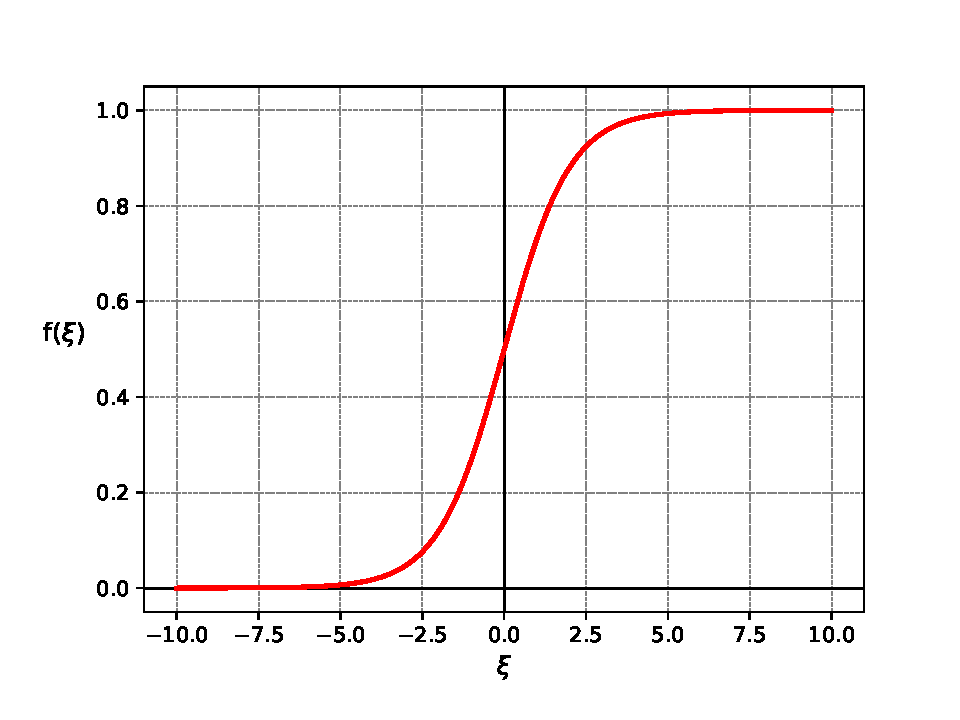
\includegraphics[width=1\textwidth]{../img/graph_sigmoid.pdf}
        \caption{Funkce \emph{sigmoid}}
        \label{fig:graph_sigmoid}
    \end{minipage}%
    \begin{minipage}{0.5\textwidth}
        \centering
        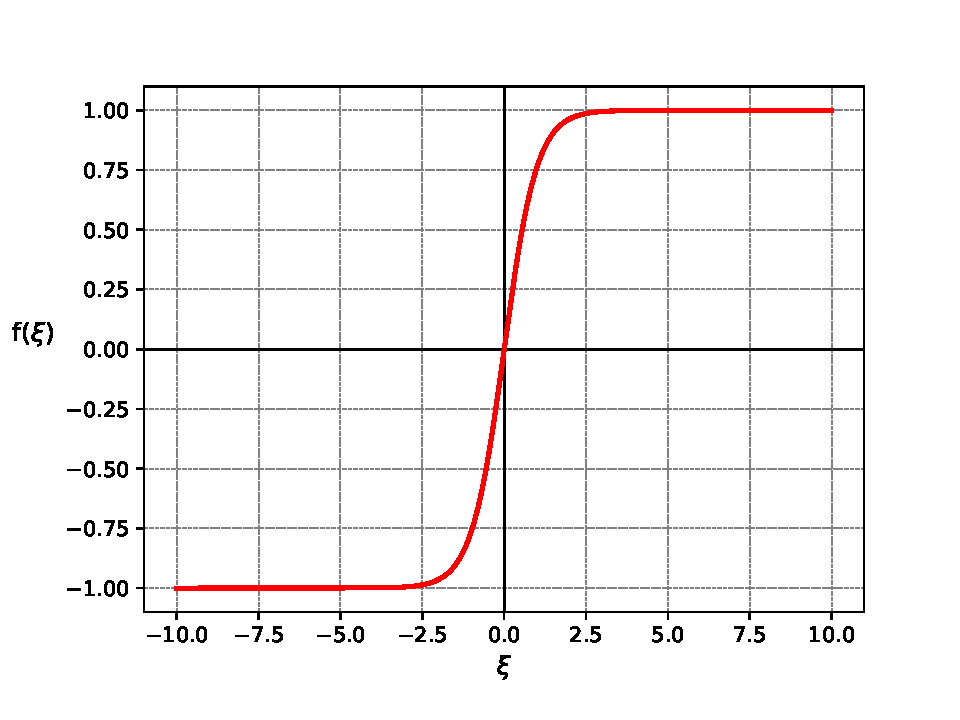
\includegraphics[width=1\textwidth]{../img/graph_tanh.pdf}
        \caption{Funkce \emph{tanh}}
        \label{fig:graph_tanh}
    \end{minipage}
    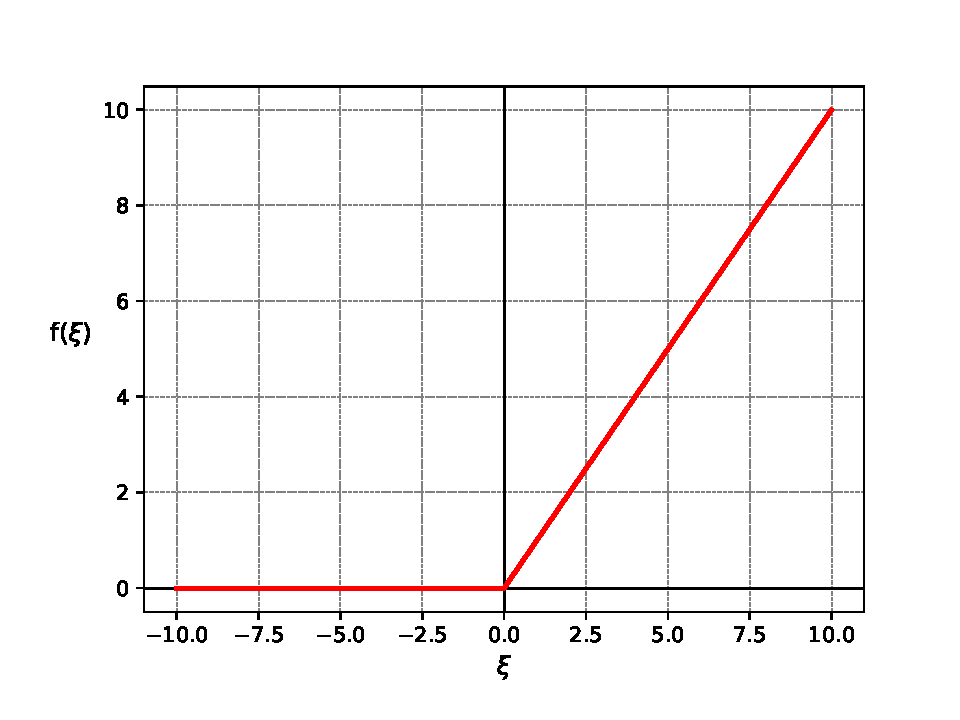
\includegraphics[width=0.5\textwidth]{../img/graph_relu.pdf}
    \caption{Funkce \emph{ReLU}}
    \label{fig:graph_relu}
\end{figure}

\paragraph{Neuronová síť}
Architektura neuronové sítě je tvořena ze třech základních typů neuronů --
vstupní (ze kterých pouze vycházejí spojení), výstupní (do kterých pouze
přicházení spojení) a skryté (spojení přicházejí a jsou předávány dál).
Neuronová síť pak jde popsat jako orientovaný graf. Pokud se jedná o graf bez
orientovaných cyklů můžeme síť označit za \emph{dopřednou neuronovou síť}.
Pokud obsahuje nějaké orientované cykly, označujeme ji jako \emph{rekurentní
neuronovou síť}. Dále se budeme zaměřovat na \emph{dopředné neuronové sítě}.

V těchto sítích vstup přechází po orientovaných hranách vrstvami neuronů, kde
každý neuron z předchozí vrstvy je spojen hranou s každým vrcholem následující
vrstvě. První vrstva se nazývá \emph{vstupní vrstva}, tvořena ze
\emph{vstupních neuronů}, a slouží pro vstup parametrů (vstupů) do sítě.
Poslední vrstva se nazývá \emph{výstupní vrstva}. Je tvořena z \emph{výstupních
neuronů} a můžeme na ní sledovat výstupy neuronové sítě. Každá
neuronová síť musí nutně mít alespoň jeden vstupní a alespoň jeden výstupní
neuron. Libovolná další vrstva mezi \emph{vstupní} a \emph{výstupní vrstvou} se
nazývá \emph{skrytá vrstva}. Těchto vrstev může být v síti teoreticky neomezené
množství.

Následující rovnice předvedou jeden dopředný průchod neuronovou sítí
přenášející vstupní vektor hodnot na výstupní vektor. V tomto příkladu si
představíme průchod dat jednoduchou sítí, skládající se ze vstupní vrstvy
(potenciál vstupních neuronů značíme $x_1,...,x_n$), jedné skryté vrstvy
neuronů (potenciály neuronů v této vrstvě označíme $h_1,...,h_k$, s
korespondujícím vektorem \emph{biasů} $b_1,...,b_k$) a výstupní vrstvy
(potenciál neuronů výstupní vrstvy $y_1,...,y_m$ opět s vektorem \emph{biasů}
$b_1,...,b_m$).

\begin{equation} \label{eq:hidden}
    h_i = f(\sum_{j}^{n} x_j w_{j,i} + b_i), \quad i = 1,...,k
\end{equation}

\begin{equation} \label{eq:output}
    y_i = a(\sum_{j}^{k} h_j w_{j,i} + b_i), \quad i = 1,...,m
\end{equation}

kde $f$ je aktivační funkce neuronů skryté vrstvy a $a$ je aktivační funkce
neuronů výstupní vrstvy. Rovnice (\ref{eq:hidden}) představuje výpočet potenciálu
neuronů ve skryté vrstvě naší neuronové sítě z příkladu a rovnice
(\ref{eq:output}) představuje výpočet potenciálů výstupních neuronů této sítě.

\paragraph{Trénování neuronových sítí}
Trénování (nebo učení) neuronových sítí je často velmi složitý proces, při
kterém se snažíme nastavit hodnoty vah jednotlivých spojů mezi neurony tak,
abychom pro konkrétní vstup na \emph{vstupní vrstvě}, dostali požadovaný výstup
na \emph{výstupní vrstvě}. 

Toto je nejčastější požadavek pro neuronové sítě při tzv. \emph{učení s
učitelem} (\emph{supervised learning}). Při tomto učení síť dostává dvojice
vektorů $(x, t)$, kde $x$ je vektor vstupních hodnot a $t$ je vektor
požadovaných výstupů. Následně se $x$ nastaví jako potenciál vstupních neuronů
a síť spočítá výstupy na výstupních neuronech. Vektor výstupních neuronů
(obvykle značený $y$) se porovná s požadovaným výstupem $t$. Na základě rozdílů
(chyby) těchto hodnot se provede úprava vah jednotlivých spojů tak, aby se při
opakovaném výpočtu sítě chyba zmenšila. Tohoto lze dosáhnout často používaným
algoritmem zpětného šíření chyby (\emph{backpropagation}), který počítá
derivace chybové funkce, aby vždy prováděl úpravy vah spojů ve směru klesající
chybové funkce.

Tento přístup ale přestává fungovat, pokud nedokážeme vytvořit vstupní
trénovací dvojice \emph{(vstup, požadovaný výstup)}, a tedy bychom nevěděli jakým
směrem váhy spojů upravovat. Toto je překážka v mnoha praktických problémech,
na které by se neuronové sítě hodilo použít. Možným řešením je nevyužívat učící
metody založené na propagaci výsledné chyby sítě, ale použít nějakou hodnotící
funkci, která ohodnotí kvalitu konfigurace dané sítě (např. po simulačním
běhu). Toto nás vede na možnost využití evolučních algoritmů pro trénovaní
neuronových sítí evolučním vývojem.

\section{Neuroevoluce} \label{NN - evolve}
Neuroevoluce \citet{Lehman:2013} je technika pro evoluční vývoj umělých
neuronových sítí pomocí principů evolučních algoritmů (popsáno v sekci
\ref{Evoluční algoritmy}). Vývoj pomocí neuroevoluce je obecnější než vývoj
pomocí klasických trénovacích metod, jelikož vývoj, na rozdíl od trénovacích
metod založených na principu \emph{učení s učitelem}, může probíhat i na sítích
proměnlivé architektury a nepotřebuje znát korektní výstupy pro daný vstup
sítě. Pro trénovaní stačí, když jsme schopni nějakým způsobem ohodnotit kvalitu
řešení, k jakému se s využitím dané konfigurace (architektura a váhy spojení)
sítě dostaneme. Díky tomuto se neuroevoluce hodí pro vývoj neuronových sítí v
případech, kdy nejsme schopni přesně určit správné výstupy sítě a pouze můžeme
pozorovat kvalitu chování daného vyvíjeného systému.

\paragraph{Vývoj neuronových sítí}
Vývoj pomocí neuroevoluce probíhá stejně jako u jiných evolučních algoritmů.
Neuronová síť je zakódovaná do genotypu jedinců, množina těchto jedinců potom
tvoří populaci, procházející vývojem skrz opakované generace. V každé generaci
je genotyp každého jedince dekódován a z těchto informací vytvořena neuronová
síť podle dekódované architektury a vah spojení. Pro každého jedince je jeho
dekódovaná síť následně otestována v testovacím prostředí, kde se ohodnotí
kvalita jedince (fitness).

Jednoduchým typem kódování může být uložení hodnot vah všech hran v neuronové
síti do jediného vektoru. Takový vektor se použije jako genotyp jedince. To
umožňuje optimalizaci vah sítě s fixní architekturou. Tento typ kódování může
být ale výpočetně velmi náročný, kvůli rychle narůstající délce genotypu s
velikostí architektury (počet vrstev a počet neuronů v síti) neuronové sítě.

\paragraph{Pokročilé metody}
S těmito problémy se můžeme potýkat hned několika způsoby. Různé styly
zakódování neuronových sítí do genotypu umožňují vývoj mnohem
rozsáhlejších sítí, zachovávající udržitelně malou velikost genetické
informace jedinců. 

Některé metody \citet{gomez2008accelerated} navrhovaly postup, jakým můžeme
omezit vývoj z celých neuronových sítí na pouze menší komponenty, které dále
mohly být spojovány dohromady s ostatními jedinci v kooperativní evoluci. To
umožnilo evoluční vývoj sítí rozsáhlejších architektur s menšími nároky na
velikost genotypu.

Jiné metody se poté zaměřily na vývoj jak vah, tak topologie neuronové sítě.
Navíc se ukázalo, že současný vývoj topologie často přináší lepší výsledky, než
vývoj pouze vah sítě. Vývoj v těchto metodách začíná s nejzákladnější
strukturou sítě, která se podle nároků problému sama vyvíjí a rozšiřuje, dokud
tyto změny přináší kvalitativní zlepšení. Často využívaným algoritmem
využívající těchto metod je algoritmus NEAT (\emph{NeuroEvolution of Augmenting
Topologies}), který si představíme v následujícím oddílu.

\subsection{NEAT} \label{NN - NEAT}
NEAT (\emph{NeuroEvolution of Augmenting Topologies})
\citep{stanley2002evolving} je neuroevoluční algoritmus vyvíjející najednou
váhy synapsí i topologii neuronové sítě, který se díky své výkonnosti stal
jedním z nejznámějších algoritmů používaných pro účely evolučního vývoje
neuronových sítí. Autoři jeho efektivitu připisují třem základním principům, se
kterými algoritmus pracuje:
\begin{enumerate}
    \item značení genetických informací pomocí tzv. \emph{historických značek},
        umožňující smysluplné křížení genotypů napříč různými topologiemi,
   \item ochrana nových genetických informací v populaci pomocí rozdělení\\
       do druhů,
    \item postupný vývoj topologie sítí od nejjednodušších struktur ke
        složitějším
\end{enumerate}
S těmito principy se NEAT ukázal jako algoritmus, který často nachází efektivní
sítě rychleji než ostatní algoritmy a výkony překonal nejlepší neuroevoluční
algoritmy pracující s neuronovými sítěmi s fixní topologií.

\paragraph{Algoritmus}
NEAT používá tzv. \emph{přímé kódování}, tedy genotyp každého jedince přímo
popisuje celou topologii sítě (všechny neurony a všechny hrany mezi neurony).
Každý genotyp obsahuje seznam \emph{genů synapsí} a seznam \emph{genů neuronů}.
Seznam genů neuronů popisuje vstupní, výstupní a skryté neurony sítě, které
mohou být spojené hranami. Každý gen synapse obsahuje následující informace:
\begin{itemize}
    \item vstupní neuron -- neuron, do kterého synapse vchází,
    \item výstupní neuron -- neuron, ze kterého synapse vychází,
    \item hodnotu váhy synapse,
    \item příznak, jestli je spojení v síti použito,
    \item \emph{historická značka} -- číslo, popisující kdy v historii
        byla daná hrana do sítě přidána; umožňuje nacházet
        odpovídající geny synapsí při křížení.
\end{itemize}
Algoritmus začíná s nejzákladnější strukturou, připomínající jednoduchý
perceptron, pouze s předem daným počtem vstupních a výstupních neuronů a
hranami mezi nimi. Tato jednoduchá topologie je rozšiřována pomocí
následujících genetických operátorů.

\paragraph{Mutace}
Mutace v algoritmu NEAT má schopnost měnit jak spojení v síti, tak její
strukturu. Mutace synapsí sítě zahrnují jednoduchou změnu váhy spojení nebo
změnu příznaku použití daného spojení v síti. Struktura sítě může mutovat
dvěma způsoby. První typ mutace přidává nový gen synapsí, spojující dva doposud
nespojené neurony. Druhý typ mutace přidává nový neuron. Tato mutace probíhá
tak, že na místo existující synapse se přidá nový neuron. Původní synapse se
označí jako nepoužívaná a namísto toho se vytvoří dvě nové rozdělující tu
původní. Váha spojení je v tomto procesu zachována. Při těchto operacích je
vždy novým genům synapsí navýšeno jejich \emph{inovační číslo} (používá
globální čítač inovací, jehož číslo je s každým novým genem navýšeno). Růst
sítí probíhá právě díky mutaci.

\paragraph{Křížení}
Křížení probíhá za pomoci \emph{inovačních čísel}. Dva jedinci se nejdříve
hranami zarovnají pomocí jejich \emph{inovačních čísel}. Stejná čísla totiž v
síti značí stejnou strukturu. Synapse, která se v obou jedincích schoduje se
dědí náhodně z jednoho rodiče. Synapse, kterou má jen jeden z rodičů se dědí z
toho lepšího z dvojce rodičů a pokud je v nějakém jedinci hrana neaktivní a v
druhém aktivní, s určitou pravděpodobností se tento stav v novém jedinci změní.
Algoritmus je tímto stylem schopný vytvářet velké množství různých topologií.
Tyto nové topologie, přestože často důležité pro řešení zadaného problému, ale
mají jen velmi malou šanci se v populaci menších topologií udržet, protože
původní menší topologie jsou na začátku často optimálnější než větší topologie.
Proto NEAT využívá systém, kterým chrání tyto nové topologie před vyhynutím z
populace.

\paragraph{Ochrana nových druhů}
Nové topologie jsou chráněny rozřazením genotypů do odlišných druhů. Jednotlivé
genotypy poté primárně soutěží s jedinci stejného druhu a nové druhy tak mají
šanci se vyvinout a optimalizovat na jejich úroveň. NEAT pro výpočet odlišností
jedinců opět využívá \emph{inovační čísla}, pomocí kterých hledá společné hrany
a vypočítá vzdálenost dvou genomů. Geny můžeme dělit do několika kategorií. Buď
se shodují a pak jsou označené jako \emph{matching genes}, nebo se neshodují.
Poté v závislosti na tom, jestli se neshodné geny objevují v rozmezí hodnot
\emph{inovačních čísel} druhého z jedinců nebo mimo toto rozmezí, nazývají se
tyto geny buď \emph{disjoint}, nebo \emph{excess}. Hodnota vzdálenosti dvou
jedinců se poté počítá jednoduchou lineární kombinací genů různých typů mezi
jedinci pomocí inovačních čísel jako

\begin{equation}
    \delta = \frac{c_1E}{N} + \frac{c_2D}{N} + c_3\cdot\overline{W}
\end{equation}

kde $N$ je celkový počet genů ve větším z jedinců, $E$ je počet \emph{excess}
genů, $D$ je počet \emph{disjoint} genů, $\overline{W}$ je průměrný rozdíl vah
shodujících se genů a koeficienty $c_1$, $c_2$ a $c_3$ umožňují nastavovat
důležitost těchto tří faktorů \citep{stanley2002evolving}.

V každé generaci se pak vytváří seznam
různých druhů a pokud se objeví genom, který nezapadá do žádného z druhů, je
pro něj vytvořen jeho vlastní nový druh.

\paragraph{Fitness}
Rozdělení do druhů má vliv i na fitness jedinců. Kvalita každého jedince se při
výpočtu fitness dělí počtem jedinců stejného druhu. To zároveň omezuje druhy v
ovládnutí celé generace a dál ochraňuje nové topologie.

\paragraph{Minimalizace dimenzionality jedinců}
Jak již bylo zmíněno, algoritmus NEAT inicializuje celou jedinců s minimální
topologií, obsahující pouze potřebný počet vstupních a výstupních neuronů,
které jsou navzájem plně propojené a žádné skryté neurony. Nové topologie
vznikají díky genetickým operátorům a všechna zvětšení genotypů jsou tedy v
evoluci opodstatněná. Díky tomuto NEAT samovolně vede k vývoji minimálních
topologií. To umožňuje, že tento algoritmus je často výkonnější než ostatní,
protože prohledává minimální potřebný prostor pro najití řešení, oproti
neuroevolučním algoritmům používající fixní topologie neuronových sítí.

\subsection{HyperNEAT} \label{NN - HyperNEAT}
Algoritmus HyperNEAT (\emph{Hypercube-based NEAT}) \citep{stanley2009hypercube}
\citep{eplex} je neuroevoluční algoritmus rozšiřující algoritmus NEAT.
HyperNEAT slouží pro vývoj umělých neuronových sítí fixní topologie (typicky
omezená tvarem hyperkrychle). 

Na rozdíl od algoritmu NEAT, používá HyperNEAT nepřímou
reprezentaci vah sítě. Tyto váhy jsou reprezentovány pomocí jiné neuronové
sítě (\emph{Compositional Pattern-Producing Network}, zkráceně \emph{CPPN}),
která jako vstup dostává pozice dvou neuronů v prostoru a vrací váhu jejich
spojení (synapse). Tímto stylem může \emph{CPPN} být využita pro reprezentaci
sítě libovolné topologie. 

Síť \emph{CPPN} je poté v algoritmu HyperNEAT vyvíjena pomocí NEAT.

Díky této nepřímé reprezentaci vah má HyperNEAT schopnost efektivně vyvinout
velmi rozsáhlé neuronové sítě s předem určenou strukturou (schopnost napodobit
regularitu velkého množství spojů v lidském mozku).

\paragraph{}
Následuje naznačení průběhu HyperNEAT algoritmu:
\begin{enumerate}
    \item Zvolit konfiguraci vyvíjené sítě (vstupní a výstupní neurony a
        rozložení skrytých neuronů),
    \item Inicializovat NEAT algoritmus s \emph{CPPN} sítěmi,
    \item Běh NEAT algoritmu, dokud není nalezeno řešení:
        \begin{enumerate}
            \item Pomocí \emph{CPPN} daného jedince vytvoř synapse pro původní
                síť,
            \item Síť otestuj v testovacím prostředí pro výpočet kvality
                řešení,
            \item S fitness hodnotami pokračuj ve vývoji genotypů popisujících
                \emph{CPPN} sítě.
        \end{enumerate}
\end{enumerate}

\section{Simulované prostředí} \label{Simulované prostředí}

% TODO: Fyzikální simulátory a sim prostředí rozlišní (\emph{fyzikální model})
++ Rozlišit simulátory

Jelikož chceme vyvíjet řízení robotů založené na interakcích s prostředím, je
pro tuto práci důležité vybrat vhodný simulátor prostředí, založený na
skutečných fyzikálních zákonech. Přáli bychom si mít možnost jednoduše
konfigurovat co nejvíce vlastností prostředí a zároveň mít co nejjednodušší
přístup k morfologii simulovaných robotů. Zároveň chceme, abychom měli možnost
do morfologie robotů nějakým způsobem zasahovat i v průběhu evolučního vývoje a
aktivně ji za běhu měnit. Jelikož plánujeme v různých prostředích provádět
experimenty s různými typy robotů, používajícími různé styly pohybu (typy
motorů, kloubů, tvarů končetin, atd.), je potřebné, aby fyzikální simulátor
(\emph{fyzikální řešič=solver}) byl schopný simulovat i složitější typy robotů.
Takovými mohou být právě třeba kráčející roboti, neboli roboti používající k
pohybu končetiny připomínající nohy, na rozdíl od jednodušších typů robotů,
kteří se mohou pohybovat pomocí kol, jejichž simulace bývá mnohdy jednodušší. 

Stejně tak, jak potřebujeme umožnit simulaci složitějších robotů, protože
nebudeme mít možnost vlastnoručně kontrolovat každý parametr, který bude při
vývoji robotům přiřazen, potřebujeme zajistit, aby fyzikální simulátor zvládal
velké rozsahy parametrů a simulace zůstala s těmito parametry stabilní. Zároveň
chceme, aby simulátor v prostředí byl deterministický, což umožní, že
předváděné experimenty můžeme dle potřeby opakovat a výsledky tak náležitě
prezentovat. 

Evoluční algoritmy jsou velmi lehce paralelizovatelné a tedy pro
urychlení procesu vývoje a experimentů bude pro nás výhodné, pokud by simulace
zvládala paralelní běh na více vláknech (více simulací, každá na vlastním
vlákně). V poslední řadě pro lehčí integraci do vlastního modulu bude užitečné,
aby modul spravující zvolený simulátor byl open-source, což nám dá volnost v
případě, že si budeme chtít chování systémů v prostředí nějak vlastnoručně
upravit.

\subsection{Simulátory prostředí}

Při hledání simulátorů prostředí, které by vyhovovali našim požadavkům a
umožňovali kontrolu a ovládání prostředí prostřednictvím zvoleného jazyka
Python, jsme narazili na několik možností. Omezený výčet těchto simulátorů zde
popíšeme -- Gazebo (v oddílu \ref{Gazebo}), Webots (v oddílu \ref{Webots}) a
CoppeliaSim (v oddílu \ref{CoppeliaSim}). Poté se pak v sekci \ref{Simulované
prostředí - f simulátory} podíváme na několik
nejpoužívanějších fyzikálních simulátorů.

\subsubsection{Gazebo} \label{Gazebo}
Gazebo \citep{gazeborobotics} je sada open-source víceplatformních knihoven pro
vývoj, výzkum a aplikaci robotů, která vznikla v roce 2002. Umožňuje kompletní
kontrolu nad simulací dynamického 3D prostředí s více agenty a generování dat
ze simulovaných senzorů. Fyzikálně korektní interakce v prostředí pak od
začátku projektu zajišťuje známý fyzikální simulátor ODE (viz sekce \ref{ODE}),
nad kterým Gazebo tvoří abstraktní vrstvu, umožňující snazší tvorbu
simulovaných objektů různých druhů. V dnešní době je stále výchozím fyzikálním
simulátorem ODE, nicméně uživatel již může vybrat celkem ze čtyř různých
fyzikálních simulátorů -- Bullet (sekce \ref{Bullet}), Simbody, Dart (sekce
\ref{Dart}) a ODE. Uživatel s knihovnou pracuje prostřednictvím grafického
rozhraní založené na knihovně Open Scene Graph používající OpenGL, nebo
prostřednictvím příkazové řádky. Prostředí a roboti mohou být tvořené buď z
grafického rozhraní prostředí, nebo v textovém formátu XML. Limitací Gazebo je
pak chybějící možnost rozdělit simulace mezi vícero vláken kvůli vnitřní
architektuře spojené s fyzikální simulací \citep{koenig2004design}. 

\subsubsection{Webots} \label{Webots}
Webots \citep{Webots} je open-source víceplatformní, robustní a deterministický
robotický simulátor vyvíjený od roku 1998, umožňující programování a testování
virtuálních robotů mnoha různých typů a jednoduchou následnou aplikaci softwaru
na reálné roboty. Simulátor je možné použít pro simulaci prostředí s vícero
agenty najednou s možnostmi lokální i globální komunikace mezi agenty. Výpočty
fyzikálních interakcí zajišťuje fyzikální simulátor ODE. Pro vývoj robotů a
prostředí je možné využít řady programovacích jazyků a to C, C++, Python, Java,
MATLAB nebo ROS (\emph{Robot Operating System}). Prostředí umožňuje práci v
grafickém rozhraní a vizualizaci simulací pomocí OpenGL. Knihovna dále nabízí
využití připravených modelů robotů, vlastní editor robotů a map a možnosti
vložení vlastních robotů z 3D modelovacích softwarů v CAD formátu
\citep{michel2004cyberbotics}.

\subsubsection{CoppeliaSim} \label{CoppeliaSim}
CoppeliaSim \citep{coppeliaSim} \citep{coppeliarobotics} (původně známý pod
jménem \emph{V-REP} = \emph{Virtual Robot Experimentation Platform}) je
víceplatformní simulační modul pro vývoj, testování a jednoduchou aplikaci
softwaru pro roboty. Dovoluje vývoj ovladačů pomocí 7 různých programovacích
jazyků a ulehčuje jejich aplikace v simulovaných a skutečných robotech.
Simulaci ovladačů je možno jednoduše rozdistribuovat mezi vícero vláken dokonce
vícero strojů, což urychluje vývoj a snižuje nároky na procesor v době
simulace. Navíc je možné vyvíjený ovladač nechat v době simulací běžet na
vlastním na dálku připojeném robotovi, co dále ulehčuje přenos finální verze
ovladačů od vývoje do skutečného světa. Prostředí umožňuje práci s širokou
řadou typů objektů, druhů kloubů, senzorů a dalších objektů obvykle používaných
při vývojích robotických ovladačů. Obsahuje lehce použitelný editor prostředí a
robotů samotných s řadou předem vytvořených modelů, které může uživatel hned
využít. Modely zároveň mohou být přidány v řadě různých formátů (XML, URDF,
SDF). Prostředí podporuje pět různých fyzikálních simulátorů (Bullet, ODE,
MuJoCo (v sekci \ref{MuJoCo}), Vortex (v sekci \ref{Vortex}) a Newton), mezi
kterými si uživatel může vybrat dle potřeb přesnosti (reálnosti), rychlosti a
dalších možností jednotlivých fyzikálních simulátorů
\citep{nogueira2014comparative}.

\subsection{Fyzikální simulátory} \label{Simulované prostředí - f simulátory}

V této podkapitole se podíváme na základní popis a možné výhody a nevýhody
jednotlivých fyzikálních simulátorů, na které jsme narazili při hledání
simulátorů prostředí.

\subsubsection{ODE} \label{ODE}
ODE (\emph{Open Dynamics Engine}) \citep{opendynamicsengine} je víceplatformní
open-source fyzikální simulátor, jehož vývoj začal v roce 2001. Je vhodný pro
simulaci pevných těles s různými druhy kloubů a pro detekci kolizí. Byl navržen
pro využití v interaktivních nebo real-time simulacích, upřednostňujících
rychlost a stabilitu nad fyzikální přesností \citep{smith2007open}. Vyžaduje
používat menší simulační kroky kvůli stabilitě. Hodí se pro simulaci vozidel,
kráčejících robotů a virtuálních prostředí. Má široké využití v počítačových
hrách a 3D simulačních nástrojích jako jsou CoppeliaSim (v sekci
\ref{CoppeliaSim}), Gazebo (v sekci \ref{Gazebo}), Webots (v sekci
\ref{Webots}) a dalších.

\subsubsection{Bullet} \label{Bullet}
Bullet je open-source fyzikální knihovna, podporující detekci kolizí a simulaci
pevných a měkkých těles. Bullet je používán jako fyzikální simulátor pro hry,
vizuální efekty a robotiku \citep{coumans}. Byl použit jako hlavní fyzikální
simulátor pro simulaci NASA \emph{Tensegrity} robotů (s vlastními úpravami pro
simulaci měkkých těles, kvůli nerealistickým metodám řešení simulace provazů)
\citep{izadi2018simulating}.

\subsubsection{Dart} \label{Dart}
Dart (\emph{Dynamic Animation and Robotics Toolkit}) je víceplatformní
open-source knihovna pro simulace a animace robotů. Od předchozích se odlišuje
stabilitou a přesností, díky zobecněné reprezentaci souřadnic pevných těles v
simulaci. Na rozdíl od ostatních fyzikálních simulátorů, aby dal vývojáři plnou
kontrolu nad simulací, umožňuje Dart plný přístup k interním hodnotám simulace.
Zároveň se díky línému vyhodnocování hodí pro vývoj real-time ovladačů pro
roboty \citep{lee2018dart}.

\subsubsection{MuJoCo} \label{MuJoCo}
MuJoCo (\emph{Multi-Joint Dynamics with Contact}) \citep{deepmind_2021} je
open-source fyzikální simulátor pro vývoj v oblasti robotiky, biomechaniky a
dalších. Často je využíváno pro testování a porovnávání různých metod
navrhování robotických systémů jako jsou třeba evoluční algoritmy nebo metody
zpětnovazebného učení \citep{salimans2017evolution}. V simulacích je pro roboty
možné nakonfigurovat využití mnoha druhů aktuátorů, včetně těch simulujících
práci svalů a k dispozici je i velké množství kloubů. Simulátor zároveň
umožňuje velký nárůst v rychlosti běhu simulace za pomoci plné podpory
paralelizace na všech dostupných vláknech a stabilitě simulace i při velmi
velkých simulačních krocích \citep{todorov2012mujoco}. Zároveň nabízí
jednoduchý styl, jakým si může uživatel konfigurovat všechny detaily simulace a
samotných simulovaných robotů pomocí jednoduchých XML konfiguračních souborů
(XML formát modelů \emph{MJCF}). V komplexním rozboru řady četně používaných
fyzikálních simulátorů byl simulátor MuJoCo hodnocen jako jeden z nejlepších co
se týče stability, přesnosti a rychlosti simulací. Další výhodou zlepšující
přesnost tohoto simulátoru je, že MuJoCo pro simulaci používá kloubní
souřadnicový systém, který předchází narušení fyzikálních pravidel a tedy
nepřesností v kloubech \citep{erez2015simulation}.

\subsubsection{Vortex} \label{Vortex}
Vortex je uzavřený, komerční fyzikální simulátor určený pro tvorbu
reálnému světu odpovídajících simulací. Obsahuje mnoho parametrů,
umožňující nastavení reálných fyzikálních parametrů dle potřeb,
většinou industriálních a výzkumných aplikací \citep{coppeliarobotics}
\citep{yoon2023comparative}.

\subsubsection{Porovnání simulátorů} \label{Simulátory - Porovnání}
V dnešní době se nám nabízí velké množství potencionálních kandidátů, vhodných
k využití pro naši aplikaci. Prakticky každý z open-source simulátorů, které
jsme našli a předvedli, by bylo možné použít pro simulaci robotů složitosti,
jakou máme předběžně v plánu. Hlavním z rozhodujících faktorů pro tento projekt
bude jak jednoduše půjde prostředí používat pro vývoj pomocí genetických
algoritmů. Chceme tedy nějaký jednoduchý přístup k simulaci a ovládání robotů,
rychlost a přesnost simulace. 

Opět většina ze simulátorů prostředí toto nabízí. Osobně se nám ale nejvíce
zalíbilo MuJoCo. Díky nedávnému otevření fyzikálního simulátoru MuJoCo a změně
prostředí (nejprve do \textbf{OpenAI Gym} a nyní do \textbf{Farama Foundation
Gymnasium}) jsme dostali možnost využít jednoduché Python API pro ovládání
robotů a zároveň konfiguraci celé simulace. 

Tato abstrakce od vlastní simulace je pro tuto práci velmi přínosná, protože se
především chceme zajímat o vývoj řízení robotů pomocí evolučních algoritmů.
Řešit zároveň složité ovladače robotů, které by se mohly lišit pro různé typy
robotů, by mohlo bezdůvodně komplikovat celý proces spojení evolučních
algoritmů s řízením robotů. Takové věci by pak mohly být problematické pro
možného uživatele, který by si chtěl sám evoluční algoritmy upravovat.

MuJoCo se zároveň ukazuje jako jeden z nejlepších volně dostupných fyzikálních
simulátorů dnes. Z výsledků článku testujících různé vlastnosti známých fyzikálních
simulátorů \citet{erez2015simulation} vychází, že MuJoCo má navrch jak v
rychlosti, tak ve kvalitě simulací. Zároveň interně využívá kloubní
souřadnicový systém, který je přesnější, protože zabraňuje nepřesnostem v
kloubech. To se hodí o to více, když v této práci chceme vyvíjet hlavně
kráčející roboty, u kterých můžeme mít i větší počty kloubů. 

Simulátor MuJoCo a roboti, které můžeme používat, je zároveň možné
jednoduše konfigurovat pomocí vlastního XML formátu a spojení s Python API
navíc umožní tyto konfigurace provádět jak často bude potřeba.

\chapter{Specifikace}

Vývoj pomocí evolučních algoritmů je možné nejlépe představit pomocí
experimentů, na kterých může uživatel sám pozorovat změny, kterými postupný
iterativní evoluční vývoj nachází možná řešení na zadaný problém. Je ale
složité vytvořit takový systém, ve kterém by uživatel mohl snadno ovládat
interní části evolučních algoritmů a tak vytvářet vlastní různorodé
experimenty. A právě tyto experimenty mohou být zásadní pro pochopení
specifických zákoutí aplikace evolučních algoritmů.

Proto cílem tohoto projektu je návrh knihovny, která by uživatelům,
přicházejících z různých oborů, umožnila bližší pochopení a seznámení se s
evolučními algoritmy pomocí vlastních interaktivních experimentů při vývoji
robotů v simulovaném prostředí. 

I jednoduché problémy, které od robotů můžeme požadovat vyřešit (např. ujití co
největší možné vzdálenosti za daný čas), poskytují pro roboty různé složitosti
(různé morfologie, počtu kloubů, atd.) dobrou představu v nárůstu obtížnosti
daného problému. Tímto zároveň experimenty s různými roboty vynucují využití
různých pokročilejších metod pro dosažení požadovaných cílů daného experimentu.

V následující sekci \ref{Specifikace-funkčnípožadavky} zabývající se funkčními
požadavky si představíme jednotlivé části, které od takového systému budeme
požadovat.

\section{Funkční požadavky} \label{Specifikace-funkčnípožadavky}

Tento projekt cílí vytvořit systém umožňující uživatelům vytvářet vlastní
experimenty s evolučním vývojem robotů v simulovaném fyzikálním prostředí.
Uživatel by měl být schopný před spuštěním experimentu podrobně pochopit a
upravit co nejvíce částí evolučního vývoje, který bude v době experimentu
probíhat. Uživatel musí být v době běhu experimentu schopný sledovat průběžné
výsledky z jednotlivých generací a vizualizovat dosavadní výsledky v
simulovaném prostředí. Po dokončení experimentu musí být možné uložit
výsledky ve formě dále zpracovatelné např. pro statistický rozbor většího
množství experimentů s možností vizualizace dat nejlepších jedinců finálních
generací.

Systém bude z hlavní části vytvořený v programovacím jazyce Python, vytvářející
uživateli přístupnější kód a umožňující rychlejší experimentování a
prototypování nápadů. Python je vhodný, jelikož se pro tento systém nesnažíme o
maximální efektivitu nebo rychlost experimentů, ale o čitelnost celého systému
a schopnost vytvářet s naší knihovnou vlastní experimenty.

Univerzálnost navrženého řešení umožní uživateli přistupovat k našemu systému
třemi způsoby popsanými níže. Každý způsob přístupu k systému má své vlastní
požadavky, které s sebou přináší. 

\paragraph{Grafické rozhraní}
Pro uživatele, kteří preferují jednoduchý přístup zprostředkovaný
interaktivním grafickým rozhraním, musí systém umožňovat vytvářet a
konfigurovat experimenty dostatečné složitosti z prostředí tohoto grafického
rozhraní. Uživatel tímto způsobem bude dále schopný pozorovat průběžné výsledky
evolučního vývoje a vizualizovat průběžná nejlepší řešení, které evoluční vývoj
najde.

\paragraph{Python knihovna}
Pro uživatele, kteří chtějí navrhovat vlastní experimenty, ale nechtějí všechno
programovat od základů. Systém pro tvorbu experimentů vývoje robotů v simulovaném prostředí bude tvořit
otevřenou Python knihovnu, kterou uživatel může připojit ke svému
projektu a pomocí naší knihovny jednoduše vytvářet experimenty s požadovanou
volností konfigurace jednotlivých parametrů evolučního vývoje.

V případě, že uživatel nebude knihovnu připojovat ke svému vlastnímu projektu,
bude systém schopen fungovat samostatně. Zároveň bude mít knihovna dostatečnou
dokumentaci na to, aby takový uživatel byl schopen provádět pokročilou
konfiguraci experimentů přímo v kódu knihovny, a aby tyto experimenty bylo
možné provádět z kódu, bez omezení výstupů systému nebo vizualizace řešení.

\paragraph{Rozšiřování knihovny}
Pro pokročilé uživatele bude navržený systém rozšiřitelnou platformou. Dokumentace
představí a vysvětlí technologie využité při vývoji této knihovny a kód
knihovny bude sestavený tak, aby byl dobře přístupný a jednoduše rozšířitelný.

\chapter{Implementace projektu} \label{chapter-implementace}
V předchozí kapitole jsme prošli funkční požadavky, očekávané od vyvíjeného
souboru programů. Následuje rozbor jednotlivých modulů, které vznikly při
vlastní implementaci. 

\paragraph{Programovací jazyk}
Celý projekt je napsána v programovacím jazyce \textbf{Python}. Cílem projektu
je vytvořit čitelnou rozšířitelnou platformu, která bude uživateli jednoduše
dostupná. Pokud uživatel bude mít potřebu vytvořené moduly jakkoli měnit nebo
rozšiřovat, implementace v Pythonu toto bez problémů umožní. Jednoduchá čitelnost Pythonu
spojená s rychlostí, jakou mohou být prováděny iterace změn, bez potřeby
zdlouhavého překladu celé knihovny, se nám zdají býti dostatečně užitečné
vlastnosti volbu Pythonu jako jazyka pro tento projekt.

\paragraph{Struktura projektu}

%TODO: Change basic imp_graph
\begin{figure}[!htb]
    \centering
    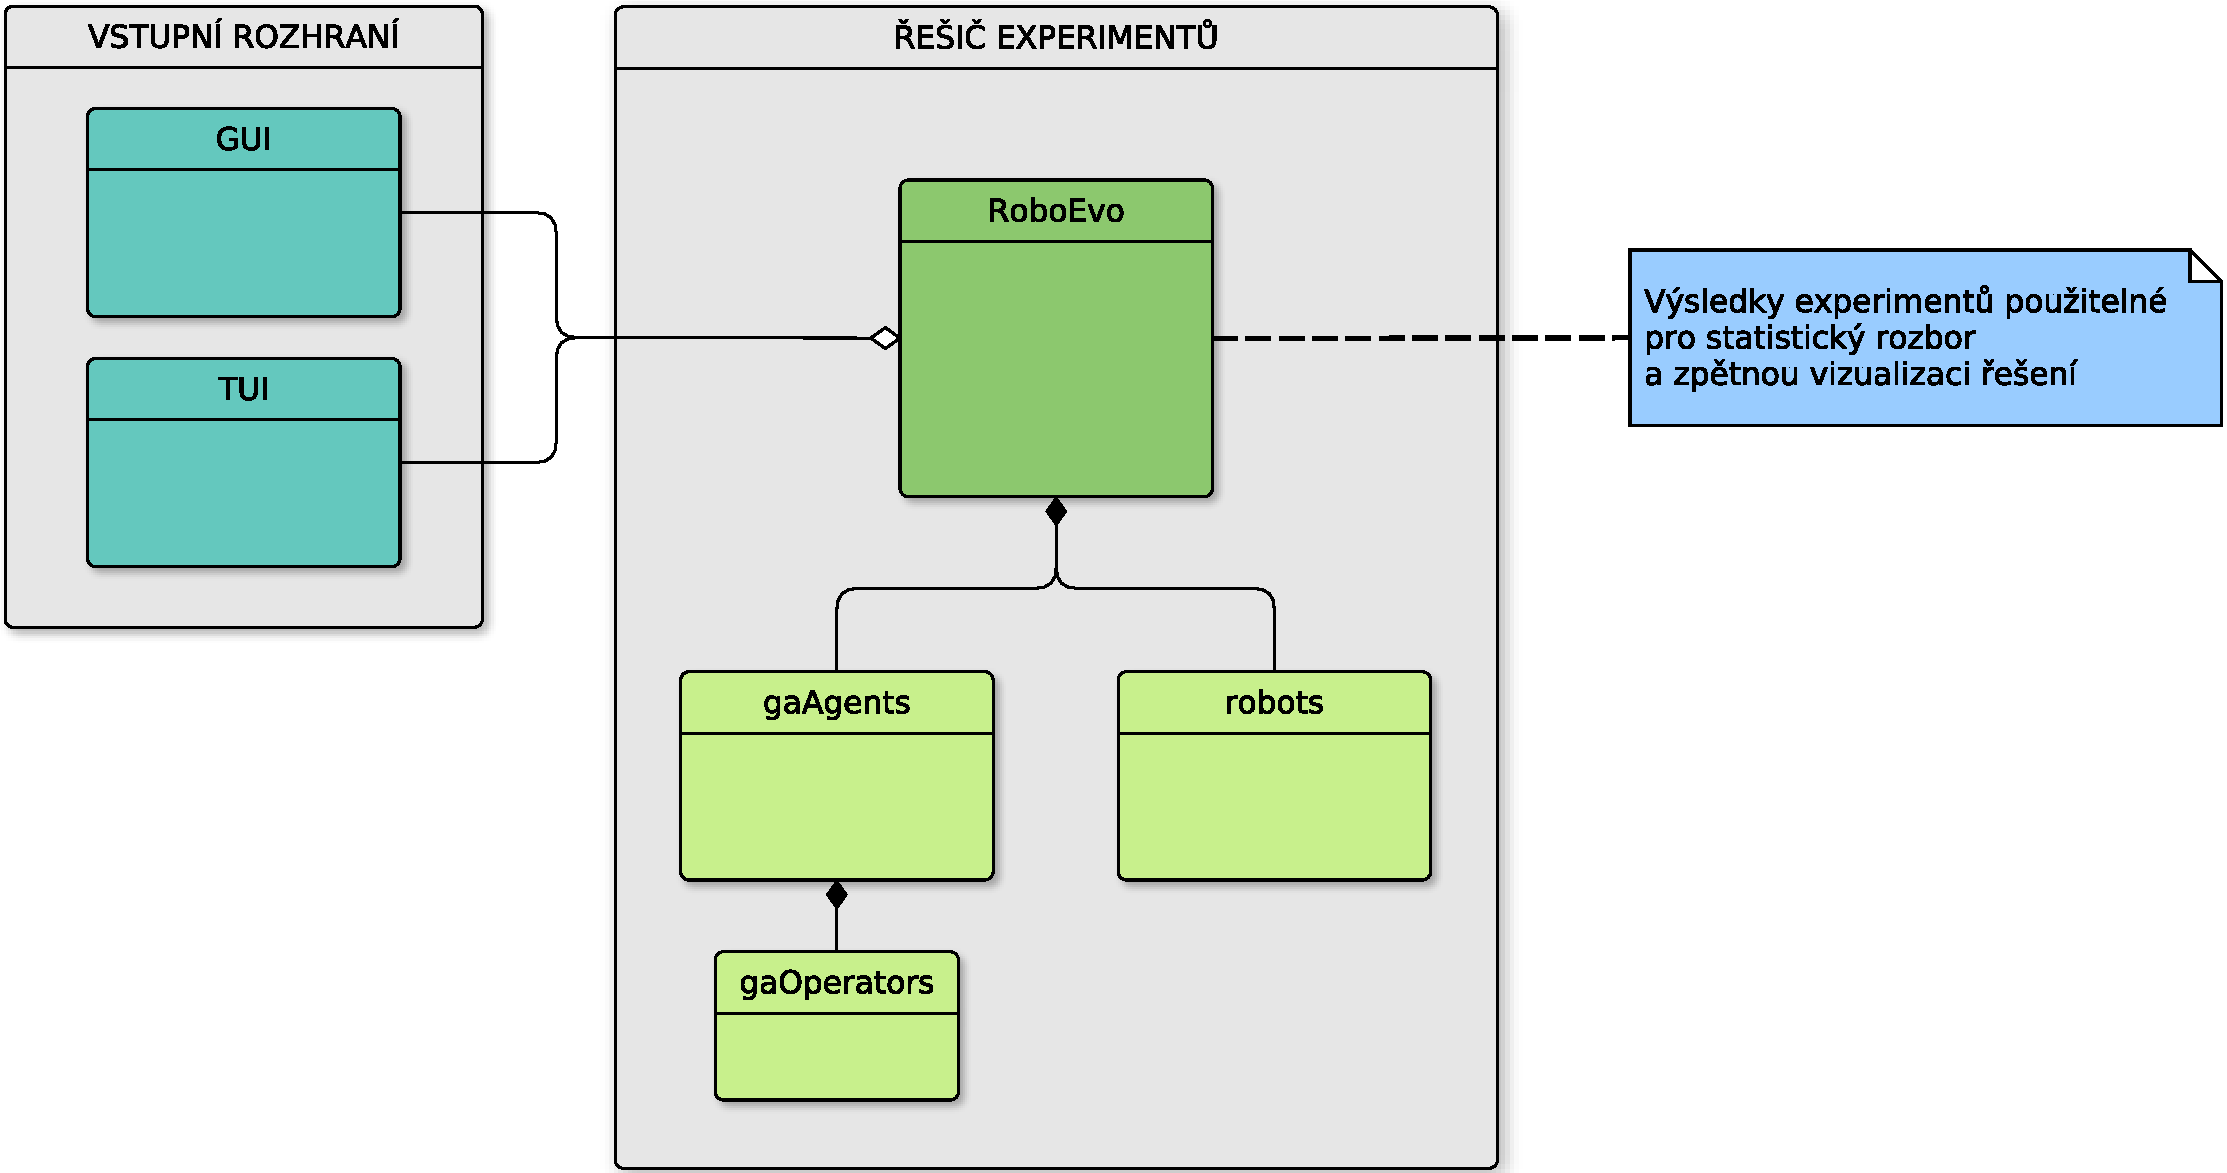
\includegraphics[width=1\textwidth]{../img/BP_imp_graph.pdf}
    \caption{Struktura projektu}
    \label{fig:struktura}
\end{figure}

Obrázek \ref{fig:struktura} popisuje na jaké části je projekt rozdělen.
Centrální částí je modul \emph{RoboEvo}, pomocí kterého knihovna provádí
evoluční experimenty. Tento modul se pro přehlednost a rozšířitelnost kódu
skládá z několika menších částí -- \emph{gaAgents} (popisující agenty a vlastní
genetické operátory) a \emph{robots} (udržující jednotný způsob přístupu k
různým robotům). 

Jak popisují funkční požadavky (v sekci \ref{Specifikace-funkčnípožadavky}),
projekt umožňuje několik možných způsobů práce s naší knihovny. Dva základní
možné přístupy jsou za pomoci grafického, nebo textového rozhraní. Tyto
přístupy jsou v projektu rozděleny do~\emph{GUI} (\emph{Graphical User
Interface}) a \emph{TUI} (\emph{Text-based User Interface}) modulů. Uživatel,
který bude chtít pracovat s kódem části knihovny zaměřené na vytváření a
provádění experimentů s evolučním vývojem, se dále může zaměřit na hlavní modul
\emph{RoboEvo} (a s ním spojené pomocné moduly).

\paragraph{} 
Dále v této kapitole v sekci \ref{imp:roboevo} popíšeme centrální modul
\emph{RoboEvo} pracující s několika dalšími pomocnými moduly, jejichž
implementace popíšeme v dalších oddílech. Představíme si modul \emph{robots}
propojující roboty ze simulátoru \emph{MuJoCo} (\emph{MuJoCo} bylo popsáno v
základních pojmech v oddílu \ref{MuJoCo}) s ostatními třídami v oddílu
\ref{imp:robots}. Dále si v oddílu \ref{imp:gaAgents} představíme třídu agentů.
Popis třídy implementující vlastní genetické operátorů se nachází v oddílu
\ref{imp:gaOperators}. V sekci \ref{imp:experimentsetter} představíme třídu
\texttt{Experiment} modulu \emph{experiment\_setter}, sloužící k uchování
a~předvolbě parametrů pro experimenty, usnadňující tak provádění většího
množství experimentů. Jako poslední si představíme moduly umožňující uživateli
práci s knihovnou buď pomocí grafického prostředí (v sekci \ref{imp:GUI}), nebo
pomocí příkazové řádky (v sekci \ref{imp:TUI}). 

\section{RoboEvo a pomocné moduly}
V této sekci popíšeme hlavní modul \emph{RoboEvo} a jeho pomocné moduly
\emph{gaAgents}, \emph{gaOperators} a \emph{robots}. Soubor těchto modulů tvoří
hlavní část celého projektu, podporující celý proces provádění evolučních
experimentů s roboty. Vytvořené rozdělení modulů bylo zvoleno pro zlepšení
čitelnosti a zjednodušení rozšiřování kódu, kde nyní každý modul
zprostředkovává velmi specifickou roli v~procesu evolučního vývoje, a tudíž je
pro uživatele jednoduché tyto části upravovat. Tato část projektu je zároveň
zcela oddělena od zpracování uživatelského vstupu, který~do hlavního modulu
vstupuje z vnějších modulů až ve chvíli zahájení experimentu. 

\subsection{Modul RoboEvo} \label{imp:roboevo}
Modul \emph{RoboEvo} je centrální modul tohoto projektu, sloužící pro spouštění
a~běh experimentů s evolučním vývojem robotů. 

Každý experiment se skládá z několika nezávislých částí. Experiment může
využívat různé typy evolučních agentů s různými genetickými operátory a může se
snažit vyvíjet různé typy robotů. Jak bylo zmíněno výše, tyto částí jsou
pro~přehlednost, čitelnost a rozšířitelnost kódu oddělené do vlastních menších
implementací, rozšiřujících hlavní modul (jednotlivé implementace budou popsány
v~dalších oddílech). Oddělené moduly umožňují jednoduše kombinovat různé agenty
s různými roboty.

\paragraph{Implementace modulu \emph{RoboEvo}}
Tento modul obsahuje funkce sloužící jak k~inicializaci evolučních experimentů,
tak k samotnému běhu evolučních algoritmů, včetně propojení s knihovnou
\emph{Gymnasium} od Farama Foundation (popsáno v sekci \ref{Simulátory -
Porovnání}), zprostředkovávající simulaci fyzikálního prostředí pro testování
jedinců.

Hlavní funkcí, která z vnějšího vstupního prostředí (např. \emph{GUI},
\emph{TUI}, vlastní modul uživatele) přijímá parametry pro spuštění
experimentů, je funkce pojmenovaná \texttt{run\_experiment}. Povinným
parametrem této funkce jsou parametry experimentu, které jsou
vloženy do jednoduché třídy \texttt{ExperimentParams} (z modulu
\emph{experiment\_params}) obsahující následující hodnoty:

%TODO: care for params changes
\begin{itemize}
    \item \texttt{robot} -- zvolený robot z modulu \texttt{robots},
    \item \texttt{agent} -- zvolený agent z modulu \texttt{gaAgents},
    \item \texttt{population\_size} -- velikost populace jedinců v
        evolučním algoritmu,
    \item \texttt{generation\_count} -- počet generací, po které bude
        evoluční algoritmus běžet,
    \item \texttt{show\_best} -- příznak určující, zda po doběhnutí evolučního
        algoritmu \\chceme v simulovaném prostředí zobrazit řešení nejlepšího
        jedince,
    \item \texttt{save\_best} -- příznak určující, zda po doběhnutí evolučního
        algoritmu \\chceme uložit nejlepšího jedince,
    \item \texttt{save\_dir} -- cesta ke složce, kam chceme uložit data z běhu
        evolučního algoritmu (pokud neexistuje, je složka automaticky vytvořena
        po doběhnutí algoritmu),
    \item \texttt{show\_graph} -- příznak určující, zda je při běhu algoritmu
        vykreslován graf zobrazující fitness hodnoty (minimální, průměrnou a
        maximální) v jednotlivých generacích,
    \item \texttt{note} -- případná poznámka, kterou může uživatel speciálně
        odlišit název dat, ukládaných po doběhnutí algoritmu.
\end{itemize}

Funkce \texttt{run\_experiment} zpracovává tyto parametry a zajišťuje vše
potřebné pro běh experimentu. V přípravě probíhá spouštění výpočetních
jednotek pro paralelizaci testovacího prostředí (umožňující ohodnocení
populace jedinců paralelně). Následně proběhne spuštění evolučního algoritmu se
zvolenými parametry, po kterém funkce uloží data vygenerovaná evolučním
algoritmem -- fitness hodnoty jedinců v každé generaci, celou
populaci jedinců z poslední generace a~(volitelné) nejlepší řešení na konci
experimentu. Tato data jsou uložená do složky, dostupné na cestě popsané v
parametru \texttt{save\_dir}.

\paragraph{Běh evolučního algoritmu}
Funkce \texttt{run\_experiment} zajišťuje spuštění evolučního algoritmu se
zvolenými parametry. Samotný běh evolučního algoritmu je poté zajištěn funkcí
\texttt{run\_evolution}. V rámci této funkce provádíme všechny kroky evolučního
algoritmu (jak byly popsány v základních pojmech evolučních algoritmů v sekci
\ref{Evoluční algoritmy}). Navíc zde pro jedince vytváříme simulační prostředí,
ve~kterých budou jedinci testováni při výpočtu fitness.

Po výpočtu fitness přichází na řadu genetické operátory, které jsou vždy
specifické pro zvolený evoluční algoritmus. V naší implementaci jsou zvolené
operátory specifikované v třídě agenta. Podrobněji třídu agentů
popíšeme v dalším oddíle \ref{imp:gaAgents}.

V rámci této funkce se zároveň sbírají důležitá data o vývoji fitness hodnot
napříč všemi generacemi a pokud to uživatel povolil, jsou aktuální data v
průběhu algoritmu vykreslována do jednoduchého grafu.

\subsection{Modul robots} \label{imp:robots}
Pro přehledné rozdělení všech částí evolučního algoritmu, zlepšení čitelnosti a
tvorby experimentů oddělujeme i třídu popisující roboty a práci s roboty do
vlastního modulu \emph{robots}. 

\paragraph{Roboti a řízení robotů}
Roboti knihovny \emph{Gymnasium} jsou popisováni pomocí XML konfiguračních
souborů, specifikující různé vlastnosti jak samotných robotů, tak prostředí, ve
kterém se pohybují. 

Robot vznikne spojováním jednoduchých tvarů pomocí kloubů. Tyto klouby mohou
být různých typů (např. pantový, kulovitý), kde každý typ se liší počtem os, ve
kterých spojeným částem těla povoluje pohyb (např. pantový v jedné ose).
Kloubu dále můžeme nastavit povolený rozsah (úhel ve stupních), ve kterém se
bude moci pohybovat. 

Následuje ukázka konfigurace pantového kloubu (\texttt{type="hinge"}) v jednom
z~výchozích robotů. Tento kloub je pohyblivý kolem osy z (\texttt{axis="0 0
1"}), interně pojmenován \texttt{hip\_1} s rozsahem od -30 do 30 stupňů.
\begin{code}
<joint axis="0 0 1" name="hip_1" pos="0.0 0.0 0.0" range="-30 30" 
 type="hinge"/>
\end{code}

Do kloubů můžeme vložit různé aktuátory, pomocí kterého můžeme kloubem
pohybovat (\emph{MuJoCo} nabízí velké množství různých aktuátorů, jejichž celý
popis je nad rámec této práce -- více informací je možné najít v oficiální
dokumentaci \emph{MuJoCo} \citep{modeling-mujocodocumentation}). 

Většina z robotů ale využívá aktuátory jen dvou typů. Prvním je \texttt{motor}
(umožňující vedle jiných specifikovat atribut převodu motoru (\emph{gear})) --
aktuátor využitý výchozím robotem \emph{AntV3} popsán později v oddílu
\ref{imp:robots.Ant}). Následuje ukázka z~XML konfigurace tohoto robota
popisující konfiguraci aktuátor motoru. Důležitým je argument
\texttt{joint}, který přiřazuje daný aktuátor ke zvolenému kloubu a argument
\texttt{ctrlrange}, který udává rozsah hodnot (nastavení aktuátoru), která~jsou
přímo mapována na povolený rozsah kloubu.
\begin{code}
<actuator>
  <motor ctrllimited="true" ctrlrange="-1.0 1.0" joint="hip_1"   
   gear="100"/>
  ...
</actuator>
\end{code}
Druhým typem je \texttt{position} (abstrakce servomotoru), umožňující nastavit
reálný atribut \texttt{kp} (\emph{velocity feedback gain}), se kterým se můžeme
potkat při nastavování PID ovladačů (\emph{proportional-integral-derivative}).
Tento aktuátor je v práci využíván v konfiguraci vlastního robota
\emph{SpotLike} (opět popsán později). Tento typ aktuátoru jsme využili,
protože \emph{SpotLike} je již složitější robot s dvanácti stupni volnosti a
možnost ručního naladění servomotorů byla nutná. To umožnilo robotovi stabilní
postoj bez příliš velkých korekcí při změnách nastavení servomotorů (jinak
vedoucích k oscilacím).

Definovaný seznam aktuátorů (část v ukázce výše) poté v simulovaném prostředí
vytváří způsob, jak robota ovládat. V pořadí, ve kterém jsme aktuátory
definovali v XML souboru, můžeme robotovi v simulovaném prostředí posílat
seznam hodnot odpovídající délky (počet aktuátorů). Aktuátory jsou následně
nastavovány na specifikované hodnoty. Tedy například robot \emph{SpotLike} s
dvanácti stupni volnosti očekává seznam dvanácti hodnot (pokud má aktuátor
nastavenou hodnotu argumentu \texttt{ctrllimited}, tak je libovolná vstupní
hodnota vždy za běhu omezena na povolený rozsah specifikovaný argumentem
\texttt{ctrlrange}).

Ovládání robota je poté sekvence n-tic reálných čísel (kde n je počet
aktuátorů), které robotovi posíláme v každém kroku simulace. Je tedy možné si
představit, jak složité je vytvořit i pro jednoduchého robota s minimálním
počtem aktuátorů takové ovládání, které ho například rozpohybuje v určitém
směru.

\paragraph{Třída \texttt{BaseRobot}}
Modul \emph{robots} je vytvořen podobným stylem jako modul \emph{gaAgents} (v sekci
\ref{imp:gaAgents}), tedy obsahuje jednu hlavní třídu \texttt{BaseRobot},
tvořící šablonu pro odvozené třídy jednotlivých robotů. Tato implementace
zásadně zjednodušuje možné připojení vlastního robota do naší knihovny což
umožní využívat vlastní roboty v experimentech s evolučním vývojem. 

Třída \texttt{BaseRobot} obsahuje několik metod využívaných všemi odvozenými
třídami a jednu abstraktní metodu, kterou každá z odvozených tříd musí
implementovat sama (informace o robotovi, sloužící k jeho prezentaci v grafické
aplikaci -- popsané v sekci \ref{imp:GUI}). Zároveň definuje všechna pole
nesoucí informace o daném robotovi (identifikační hodnota \emph{MuJoCo}
prostředí, slovník jmen částí těla robota, které mohou být použité při
evolučním vývoji a odkaz na náhledový obrázek, zobrazující robota, pro
\emph{GUI}). Tyto informace jsou uložené o každém robotovi voláním
konstruktor rodičovské třídy s potřebnými parametry.

Následuje seznam veřejných metod základní třídy
\texttt{BaseRobot}:

\begin{itemize}
    \item \texttt{create(body\_part\_mask, individual, tmp\_file = None)}
        -- metoda,\\která na vstupu dostane argument masky částí těla
        popisující, které části budou moci být měněny evolučním algoritmem
        (seznam hodnot -- buď hodnoty \texttt{False}/0 pro části těla, které se
        nemají měnit, nebo specifikování rozsahu ve formátu \texttt{tupple} --
        \texttt{(min, max)}) a argument jedince, ze kterého získává délky části
        těla daného jedince (používané při vývoji morfologie robota). Tyto
        hodnoty metoda použije při úpravě konfiguračního XML souboru, který
        popisuje robota v simulačním prostředí, a vrací nově vytvořený soubor s
        konfigurací (pokud metoda dostane argument \texttt{tmp\_file}, tak
        konfiguraci vygeneruje do tohoto souboru),
    \item \texttt{create\_default()} -- stejná funkcionalita jako předchozí
        metoda, ale pro zjednodušení zápisu vytvoří konfiguraci robota s
        výchozím nastavením,
    \item \texttt{body\_part\_names()} -- metoda vracející jména všech
        dostupných končetin robota.
\end{itemize}

\paragraph{Konfigurace vlastního robota}
Roboti v simulátoru \emph{MuJoCo} jsou popisování konfiguračními soubory ve
formátu XML (dokumentace k modelování v \emph{MuJoCo}
\citep{modeling-mujocodocumentation}). Pro naši implementaci využíváme tento
formát pro tvorbu šablony konfiguračních souborů, kde na místo některých
číselných hodnot v konfiguraci můžeme dosadit speciální značky, které naší
knihovně umožní konfigurační soubor upravovat za běhu algoritmu. Toto nám
umožní vytvářet experimenty, které vedle pohybu mohou zároveň vyvíjet i
morfologii robotů (např. velikost specifikovaných končetin). 

Speciální značky mohou být ve tvaru např \texttt{\$L\_FRONT(0.75)\$} nebo
\texttt{@...@}. 

Značka ohraničená symbolem $\$$ se může nacházet na pozici teoreticky libovolné
číselné hodnoty v konfiguračním souboru. Značka označuje a pojmenovává hodnotu
(zde např. interně pojmenovaná jako \texttt{L\_FRONT} s výchozí hodnotou
$0.75$), kterou bude možno zvolit pro vývoj pomocí evolučního algoritmu. 

Značka ohraničená symbolem $@$ označuje část konfiguračního souboru, která může
obsahovat základní aritmetické operace, které budou vyhodnoceny po dosazení
hodnot za všechny značky ohraničené symbolem $\$$. Umožňuje tedy provádět
jednoduché výpočty v konfiguračních souborech.

Značky jsou při vytváření robota vyhledávány pomocí regulárních výrazů
očekávajících značky předvedeného formátu.

Pokud máme vytvořenou konfiguraci robota v XML souboru (např. soubor
\emph{custom\_stick\_ant.xml}), můžeme robota jednoduše přidat mezi použitelné
roboty, vytvořením odpovídající třídy v modulu \emph{robots} (podle následující
ukázky -- tvorba robota \emph{StickAnt}). Tato třída dále potřebuje určit cestu
k náhledovému obrázku (v tomto případě \emph{Basic-Ant.jpg}) a identifikační
název \emph{MuJoCo} prostředí, ve kterém bude robot testován (nyní všichni
roboti využívají stejné prostředí -- \emph{custom/CustomEnv-v0}).

\begin{code}
class StickAnt(BaseRobot): # tvorba robota StickAnt
    def __init__(self):
        # všechny soubory se nachází ve stejné složce jako 
        # tento modul
        DIR = os.path.dirname(__file__)

        # cesta k šabloně konfiguračního souboru robota
        source_file = DIR+"/custom_stick_ant.xml"

        # cesta k náhledovému obrázku robota
        picture_path = DIR+"/Basic-Ant.jpg"


        # MuJoCo prostředí, ve kterém robot bude spuštěn
        environment_id = "custom/CustomEnv-v0"

        # 'custom/CustomEnv-v0' označuje naše prostředí 
        # vytvořené tak, aby jednoduše podporovalo všechny základní 
        # druhy robotů (bez robotů využívající NEAT)

        # volání inicializační funkce třídy BaseRobot,
        # která drží všechny informace v jednotném formátu
        super(StickAnt, self).__init__(source_file, 
                                       picture_path, 
                                       environment_id)

    # implementace vlastní abstraktní metody pro popis robota pro GUI
    @property
    def description(self):
        return """ Libovolně rozsáhlý popis robota """
\end{code}

\subsubsection{Implementovaní roboti}
Knihovna obsahuje tři implementované roboty. Roboti by měli být dostatečně
rozdílní v obtížnosti ovládání, aby se na nich mohl demonstrovat rozdíl v
efektivitě pokročilých evolučních algoritmů.

\paragraph{Robot \emph{StickAnt}} \label{imp:robots.StickAnt}
Základním robotem je robot pojmenovaný \emph{StickAnt} (ukázka na obrázku
\ref{imp:fig:robots.StickAnt}). Výchozím robotem pro jeho tělo je výchozí
\emph{AntV3} z knihovny \emph{Gymnasium}. Morfologie tohoto robota je velmi
jednoduchá. Jeho tělo se skládá z koule fungující jako torso a čtyř
jednoduchých končetin, kde každá je jedním pantovým kloubem připojena na torso.
\begin{figure}[!htb]
    \centering
    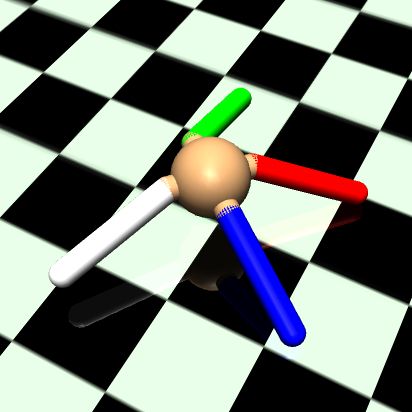
\includegraphics[width=0.4\textwidth]{../img/crop_Basic-Ant.jpg}
    \caption{Robot \emph{StickAnt}}
    \label{imp:fig:robots.StickAnt}
\end{figure}

\paragraph{Robot \emph{AntV3}} \label{imp:robots.Ant}
Jedná se o výchozího robota knihovny \emph{Gymnasium} (ukázka na obrázku
\ref{imp:fig:robots.AntV3})). Morfologie tohoto robota je pokročilejší než
morfologie robota \emph{StickAnt}. Každá noha má navíc jeden pantový kloub,
který můžeme brát jako koleno. Ovládání tohoto robota již začíná být
složitější, kvůli tomu, že robot se může převrátit a spadnout.
\begin{figure}[!htb]
    \centering
    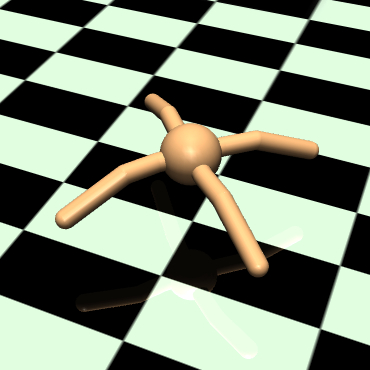
\includegraphics[width=0.4\textwidth]{../img/crop_Ant-v3.jpg}
    \caption{Robot \emph{AntV3}}
    \label{imp:fig:robots.AntV3}
\end{figure}

\paragraph{Robot \emph{SpotLike}} \label{imp:robots.Spot}
Robot inspirovaný pokročilým robotem pojmenovaným \emph{Spot} od firmy
\emph{Boston Dynamics} (popsaný v článku \citep{guizzo2019leaps}). Jedná se o
čtyřnohého robota s morfologií těla, která připomíná psa (ukázka na obrázku
\ref{imp:fig:robots.SpotLike}). Každou nohu ovládají tři klouby (dohromady tedy
12 stupňů volnosti pro celého robota), což z tohoto robota dělá toho
nejobtížnějšího na ovládání. Čtyři vysoké nohy jsou zároveň vratké a tudíž je o
to těžší vyvinout stabilní pohyb, který ho udrží nepadat.

\begin{figure}[!htb]
    \centering
    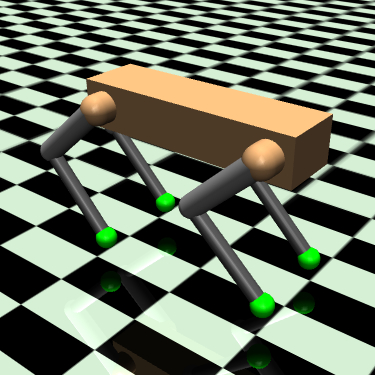
\includegraphics[width=0.4\textwidth]{../img/crop_SpotLike.jpg}
    \caption{Robot \emph{SpotLike}}
    \label{imp:fig:robots.SpotLike}
\end{figure}

\paragraph{}

\paragraph{Roboti knihovny Gymnasium}
Naše knihovna umožňuje jednoduché přidání robotů, volně dostupných v knihovně
Gymnasium. Většina těchto robotů má ve~svém prostředí definované složitější
cíle, kterých mají dosáhnout (např. balancování kyvadla ve vertikální poloze).
Tato prostředí jsou často smysluplně využitelná pouze pro experimenty s vývoj
pomocí algoritmů neuroevoluce. Několik vybraných robotů jsou jako ukázky již
implementováni v naší knihovně -- \emph{Walker2D}, \emph{InvertedPendulum},
\emph{InvertedDoublePendulum}.

\subsection{Modul \emph{gaAgents}} \label{imp:gaAgents}
Modul \emph{gaAgents} je kolekcí několika tříd popisující agenty využívané
evolučními algoritmy. Každá třída agenta povinně obsahuje několik funkcí, které
specifikují jak vypadá genotyp jedinců vytvořených podle tohoto agenta, jakým
způsobem se generuje populace takových jedinců, jaké genetické operátory budou
při~evolučním vývoji použité a jakým stylem probíhá transformace genotypu
jedince na nastavení odpovídajících aktuátorů robota. Agent zároveň uchovává
informaci o zvoleném typu evoluce, který určuje, zda evoluční algoritmus může
vyvíjet řízení robota, jeho morfologii nebo obojí.

Agent pro evoluční algoritmus vytváří jedince, jejichž genotyp se skládá ze
dvou vektorů. První z vektorů vždy obsahuje hodnoty, pomocí kterých agent
generuje na základě vstupu z testovacího prostředí odpovídající nastavení pro
aktuátory robota. Druhý z vektorů obsahuje hodnoty popisující délku těch částí
těla robota, u kterým jsme povolili jejich vývoj pomocí evolučního algoritmu.
Pokud jsme nepovolili vývoj žádné části těla, tento vektor zůstane prázdný.

\paragraph{Třída agenta}
Hlavní třídou tohoto modulu, tvořící šablonu pro všechny další definované
agenty, je třída \texttt{BaseAgent}. Všechny třídy popisující agenty mají
povinnost odvozovat od této třídy základního agenta. Součástí této třídy je
několik abstraktních metod (metody, které odvozená třída má povinnost
implementovat, aby byla použitelná). Výčet abstraktních metod agenta:

\begin{enumerate}[a)]
    \item metody využívané evolučním algoritmem:
        \begin{itemize}
            \item \texttt{generate\_population(population\_size)} -- metoda
                vytvářející populaci jedinců požadované velikosti,
            \item \texttt{get\_action(individual, step)} -- metoda
                zprostředkovávající transformaci části genotypu jedince
                (kterou funkce získá ze vstupního parametru \texttt{individual}) na
                nastavení pro aktuátory daného robota na základě vstupu z
                testovacího prostředí (simulační krok v testovacím prostředí --
                z parametru \texttt{step}),
            \item \texttt{selection(population, fitness\_values)} -- genetický
                operátor -- metoda s parametry populace jedinců a jejich
                fitness hodnotami, která nějakým způsobem (s využitím
                genetických operátorů selekce) vybere jedince a vrátí jejich
                seznam,
            \item \texttt{crossover(population)} -- genetický operátor --
                metoda s parametrem populace jedinců (označující skupinu
                rodičů), na které provede křížení genotypů a vrátí vytvořenou
                skupinu potomků,
            \item \texttt{mutation(population)} -- genetický operátor -- metoda
                do které jako parametr vstoupí skupina jedinců (potomků
                křížení), na kterých provede mutaci genotypu a vrátí
                zmutované potomky,
            \item \texttt{switch\_evo\_phase()} -- metoda využívána z hlavního
                modulu, který řídí evoluční algoritmus, sloužící pro vyhlášení
                změny typu evolučního vývoje (přechod mezi vývojem řízení a
                morfologie při odděleném vývoji řízení a~morfologie),
        \end{itemize}
    \item metody využívané pro vstupní rozhraní:
        \begin{itemize}
            \item \texttt{description()} -- metoda, do které můžeme vložit
                text, sloužící jako rozsáhlejší popisek agenta v \emph{GUI}.
        \end{itemize}
\end{enumerate}

Využití abstraktních metod se pro tuto implementaci hodí, protože tímto
způsobem můžeme v experimentech jednoduše zaměňovat typy využívaných
agentů a měnit tak průběh evolučního vývoje. 

\paragraph{Vlastní agent}
Uživatel může jednoduše přidávat vlastní agenty, vytvořením třídy odvozené
od třídy \texttt{BaseAgent} a implementováním potřebných metod. Pro
zjednodušení tohoto procesu, uživatel nemusí vlastnoručně programovat všechny
tyto metody, ale může využít připravené genetické operátory, implementované v
pomocném modulu \emph{gaOperators}, který si představíme v následujícím oddílu
\ref{imp:gaOperators}. Pokud uživatel nenajde takovou funkci, která by přesně
odpovídala jeho požadavkům, může si potřebný algoritmus dopsat sám, za dodržení
pravidel specifikovaných implementací třídy agenta.

\paragraph{Existující agenti}
V následujícím seznamu krátce představíme všechny dostupné agenty připravené
pro experimenty:

\label{imp:gaAgents.stepcyclehalfagent}
\label{imp:gaAgents.sinefuncfullagent}
\label{imp:gaAgents.sinefunchalfagent}
\label{imp:gaAgents.stepcyclehalfagent}
\label{imp:gaAgents.TFSagent}
\begin{itemize}
    \item \textbf{\emph{StepCycleHalfAgent}} -- agent, jehož genotyp je vektor předem
        zvolené délky pro polovinu aktuátorů robota, kde hodnoty v genotypu přímo
        popisují hodnoty nastavení aktuátorů. Tato nastavení jsou periodicky
        opakována v periodě zvolené délky vždy pro polovinu aktuátorů a pro
        druhou polovinu jsou symetricky přenesena a nastavena na opačné
        hodnoty (vynásobením hodnoty minus jedničkou -- všechny aktuátory mají
        povolený rozsah hodnot od $-1$ do $1$).

    \item \textbf{\emph{StepCycleFullAgent}} -- agent, podobný agentovi
        \emph{StepCycleHalfAgent}, generující do svého genotypu nastavení pro
        všechny aktuátory robota pro~určitý počet kroků. Tato nastavení se opět
        periodicky opakují.

    \item \textbf{\emph{SineFuncFullAgent}} -- agent, jehož genotyp popisuje
        parametry sinusové funkce pro každý aktuátor robota (amplituda,
        frekvence, posun v ose $x$ a posun v ose $y$). Nastavení aktuátorů je
        pak vygenerované výpočtem sinus funkce pro každý aktuátor v daném
        simulačním kroku (z celočíselného parametru\texttt{step} funkce
        \texttt{get\_action}), podle následující rovnice:
        \begin{equation}
            \text{nastavení aktuátoru} = f(step) = A\cdot\sin(\frac{2\pi\cdot step}{T} + \delta_x) + \delta_y
            \label{sinefunc}
        \end{equation}
        kde $T$ je perioda sinus funkce, $A$ je amplituda funkce a $\delta_x$ a
        $\delta_y$ jsou její posuny. Hodnota parametru \texttt{step} může být
        pro plynulejší přechody mezi nastaveními aktuátorů dělena na menší
        hodnoty.

    \item \textbf{\emph{SineFuncHalfAgent}} -- agent, podobný jako
        \emph{SineFuncFullAgent}, který má parametry sinusových funkcí pouze pro
        polovinu aktuátorů. Druhou polovinu generuje opět přenesením opačných
        hodnot z první poloviny. Pro výpočet hodnoty nastavení aktuátorů
        využívá stejné funkce, jako \emph{SineFuncFullAgent} (funkce
        (\ref{sinefunc})).

    \item \textbf{\emph{TFSAgent}} -- složitější agent než \emph{SineFuncFullAgent},
        využívající genotyp popisující zkrácenou Fourierovu transformaci pro
        každý aktuátor na generování požadovaného nastavení. Genotyp obsahuje
        parametry pro amplitudy a posuny pro vybraný počet sinus funkcí.
        Výpočet nastavení jednoho aktuátoru potom vypadá dle následující
        funkce (\ref{TFS_func}):

        \begin{equation}
            \text{nastavení aktuátoru} = f(step) = \sum_{i=1}^{N}A_i\cdot\sin\frac{i\cdot
            step\cdot2\pi}{T} + \delta_i
            \label{TFS_func}
        \end{equation}
        kde $N$ je pevný počet sinus funkcí, na které součet omezíme, $T$ je
        pevně zvolená perioda, $A_1,...,A_N$ jsou amplitudy sčítaných
        sinusoid a $\delta_i,...,\delta_N$ jsou jejich posuny,
    \item \textbf{\emph{NEATAgent}} -- agent, implementující algoritmus
        neuroevoluce -- NEAT (\emph{NeuroEvolution of Augmenting Topologies}),
        popsaný v základních pojmech v sekci \ref{NN - NEAT}. Naše implementace
        využívá python knihovnu pro NEAT -- \emph{neat-python}
        \citep{McIntyre_neat-python}.
\end{itemize}

Kromě zcela náhodného agenta a agenta využívajícího NEAT, se agenti snaží pro
urychlení evolučního vývoje předpokládat, že vhodné řešení bude v podobě
nějakého periodického pohybu a generují tedy výstupy pro nastavení aktuátorů
podle nějakých periodických funkcí. 

\subsection{Modul gaOperators} \label{imp:gaOperators}
Modul \emph{gaOperators} slouží pro usnadnění tvorby evolučních algoritmů
implementací řady nejpoužívanějších genetických operátorů použitelných v
metodách agentů (popsaných v předešlé sekci \ref{imp:gaAgents}). 

Seznam implementovaných operátorů (podrobný popis operátorů v sekci
\ref{Evoluční algoritmy - operátory}):
\begin{itemize}
    \item \texttt{roulette\_selection(pop, fitness\_values)} -- implementace
        \emph{ruletové selekce}, s argumenty populace jedinců a jejich fitness
        hodnoty. Vyžaduje, aby~všechny hodnoty \texttt{fitness\_values} byly
        nezáporné,
    \item \texttt{tournament\_selection(pop, fitness\_values, k)} --
        implementace \emph{turnajové selekce}, s argumenty populace
        jedinců, jejich fitness hodnoty a hodnotu $k$ určující velikost turnaje,
    \item \texttt{tournament\_prob\_selection(pop, fitness\_values, prob, k)}
        -- implementace pokročilé \emph{turnajové selekce}, kde umístění
        jedince v turnaji mezi $k$~náhodně vybranými jedinci určuje jeho
        pravděpodobnost na zvolení podle vzorce: 
        \begin{equation}
            p(X) = prob\cdot(1-prob)^{(X-1)}
        \end{equation}
        kde $X=1,...,k$ je pozice, na které se daný jedince umístil v turnaji a $prob$
        je vstupní parametr funkce, určující pravděpodobnost na zvolení
        prvního. Toto rozdělení pravděpodobností je normalizováno tak, aby pro
        každou volbu $k$ se sečetlo na jedničku. Následně je vektor
        pravděpodobností využit při náhodném výběru jednoho z jedinců v
        turnaji, 
    \item \texttt{crossover\_uniform(pop, agent)} -- implementace základního
        operátoru uniformního křížení, popsaného v sekci \ref{Evoluční
        algoritmy - operátory}, s argumenty populace jedinců a odkazem na
        zvoleného agenta, který pro metody udržuje další potřebné informace
        (např. sílu mutace jedinců, příznak označující povolení vývoje
        morfologie),
    \item \texttt{crossover\_single\_point(pop, agent)} -- implementace
        operátoru jednobodového křížení, popsaného v sekci \ref{Evoluční
        algoritmy - operátory},
    \item \texttt{uniform\_mutation(pop, agent)} -- implementace jednoduchého
        operátoru uniformní mutace (popsané v sekci \ref{Evoluční algoritmy -
        operátory}), využívající parametry agenta, který specifikuje
        pravděpodobnost mutace samotného jedince, pravděpodobnost mutace akcí a
        pravděpodobnost mutace částí těla (\emph{individual mutation
        probability}, \emph{action mutation probability}, \emph{body mutation
        probability}),
    \item \texttt{uniform\_shift\_mutation(pop, agent)} -- implementace
        upraveného operátoru uniformní mutace, využívajících stejných parametrů
        pravděpodobností jako předchozí operátor \texttt{uniform\_mutation}.
        Tento operátor provede mutaci dané hodnoty vygenerováním hodnoty malé
        změny z povoleného rozsahu (příklad -- náhodně zvolená
        $\delta\in[\frac{min}{0.05}, \frac{max}{0.05}]$), kterou přičte k
        původní mutované hodnotě ($a = a' + \delta$, kde $a'$ je mutovaná
        hodnota před mutací a $a$ hodnota po aplikování mutace). Výsledná
        hodnota je poté omezena do povoleného rozsahu.
\end{itemize}

\section{Třída experimentů} \label{imp:experimentsetter}
Pro usnadnění vytváření, ukládání a výběru experimentů jsme v modulu
\emph{experiment\_setter} implementovali vlastní jednoduchou třídu
\texttt{Experiments}. Tato~třída má za úkol být seznamem nadefinovaných
experimentů, které mohou být rychle načteny buď podle zvoleného názvu
experimentu, nebo podle jména funkce, vytvářející experiment.

Hlavní datovou strukturou třídy je slovník, který má jako klíče názvy
experimentů a jako hodnoty korespondující parametry experimentu (objekt třídy
\texttt{ExperimentParams}). Tento slovník je naplněn v době inicializace třídy
a uživatel do něj může přidat vlastní experimenty (je potřeba vytvořit záznam
ve slovníku experimentů s hodnotou odpovídajících parametrů experimentu).

Třída \texttt{Experiments} obsahuje, všechny experimenty předvedené v této
práci, ze kterých uživatel může brát inspiraci při vytváření vlastních. Samotný
experiment je popsán vždy ve vlastní funkci vracející parametry experimentu.
Jak může vypadat tvorba experimentu můžeme vidět v následující ukázce.

\begin{code}
def exp10_TFS_spotlike(self, run=True):
    robot = robots.SpotLike()
    agent = gaAgents.TFSAgent(robot, ...)
    note = "exp1.0"

    # __create_batch_dir - Funkce, která na základě zvoleného robota, 
    # agenta a zvolené poznámky vytvoří cestu, kam se uloží 
    # výsledky experimentu.
    batch_dir = self.__create_batch_dir(robot, agent, note) 

    # tvorba parametrů experimentu
    params = ExperimentParams(robot, 
                              agent,
                              population_size=100,
                              generation_count=500,
                              show_best=False,
                              save_best=True,
                              save_dir=batch_dir,
                              note="")

    # pokud je experiment tvořen přímo voláním funkce, vypiš info
    if run: 
        self.__exp_start_note()

    return params
\end{code}

Tato třída výrazně usnadňuje spouštění experimentů pro vstupní prostředí. Navíc
díky dalším metodám (pro kontrolu správného výběru experimentu a pro výpis
všech vytvořených experimentů) uživatel může pracovat s experimenty,
aniž~by měl potřebu znát obsah této třídy.

\section{Grafické rozhraní} \label{imp:GUI}
Pro nastavování a spouštění experimentů může uživatel využít jednoduché
grafické aplikace. Tento přístup je vhodný zejména pro prototypování nápadů na
experimenty. Uživatel v aplikaci může rychle vybírat a měnit parametry jak
agentů, robotů, tak samotného genetického algoritmu. Oproti tomu, použití
grafického rozhraní nemusí být vhodné v případech, že uživatel bude chtít
provádět větší množství předem připravených experimentů, při kterých běh
grafického rozhraní není potřeba.

\paragraph{Implementace GUI}
Implementace používá modul \emph{PySimpleGUI} \citep{pysimplegui}, umožňující
jednoduchý a rychlý vývoj grafických aplikací v Pythonu. 

\emph{PySimpleGUI} umožňuje vytvářet prvky rozhraní (např.
tlačítka, vstupní textová pole, ale i celá okna) uvnitř vlastních funkcí a
prvky pak vracet jako hodnotu funkce. To oproti jiným grafickým knihovnám
zlepšuje celkovou čitelnost a přehlednost kódu. Prvky rozhraní musí být v okně
vložené do rozložení~(\emph{layout}). Tato rozložení ale mohou být jednoduše
uložená v seznamech, díky schopnosti Pythonu pracovat se seznamy
heterogenních dat.

Naše grafická aplikace je rozdělená do několika sekcí:

% TODO: Change pics
\begin{itemize}
    \item \emph{Main} -- přehled informací o nastavovaném experimentu a
        spouštění experimentu (ukázka na obrázku \ref{imp:fig:GUI_main}),
    \item \emph{Robot select} -- sekce pro výběr robota (ukázka na obrázku
        \ref{imp:fig:GUI_robot}),
    \item \emph{Agent config} -- sekce pro výběr a nastavení parametrů agenta
        (ukázka na obrázku \ref{imp:fig:GUI_agent}),
    \item \emph{Evolution config} -- podrobnější úprava genetických operátorů a
        parametrů evolučního algoritmu (ukázka na obrázku \ref{imp:fig:GUI_evo}).
\end{itemize}

\begin{figure}[!htb]
    \centering
    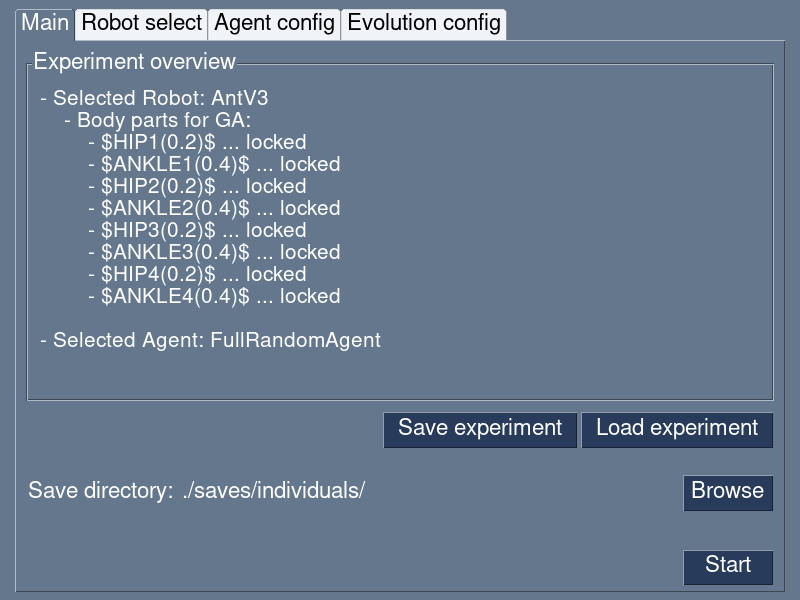
\includegraphics[width=0.6\textwidth]{../img/GUI_main_tab.jpg}
    \caption{Úvodní okno aplikace}
    \label{imp:fig:GUI_main}
\end{figure}
\begin{figure}[!htb]
    \centering
    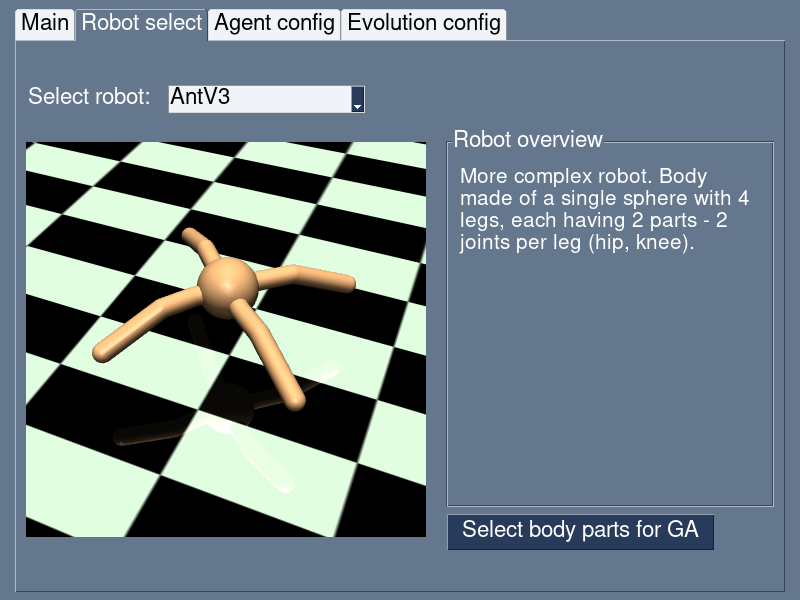
\includegraphics[width=0.6\textwidth]{../img/GUI_robot_tab.jpg}
    \caption{Okno pro volbu robota pro experiment}
    \label{imp:fig:GUI_robot}
\end{figure}
\begin{figure}[!htb]
    \centering
    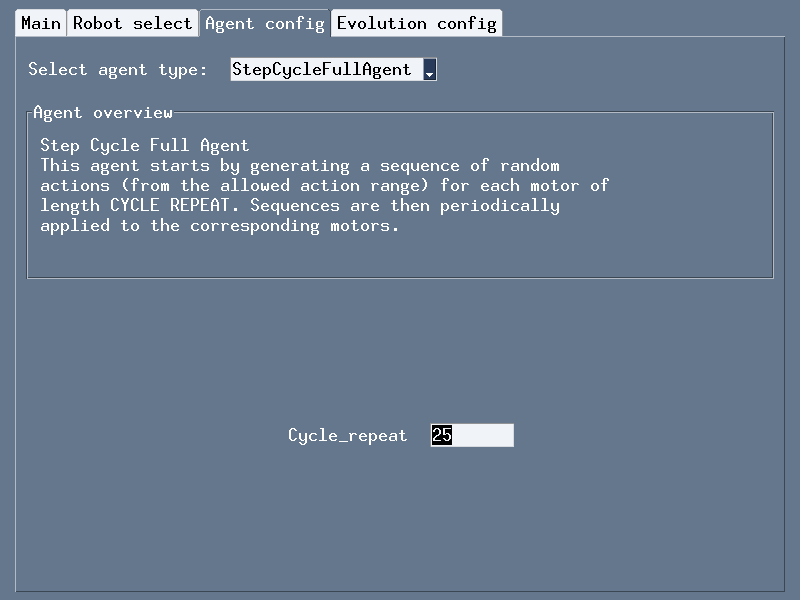
\includegraphics[width=0.6\textwidth]{../img/GUI_agent_tab.jpg}
    \caption{Okno pro volbu agenta pro experiment}
    \label{imp:fig:GUI_agent}
\end{figure}
\begin{figure}[!htb]
    \centering
    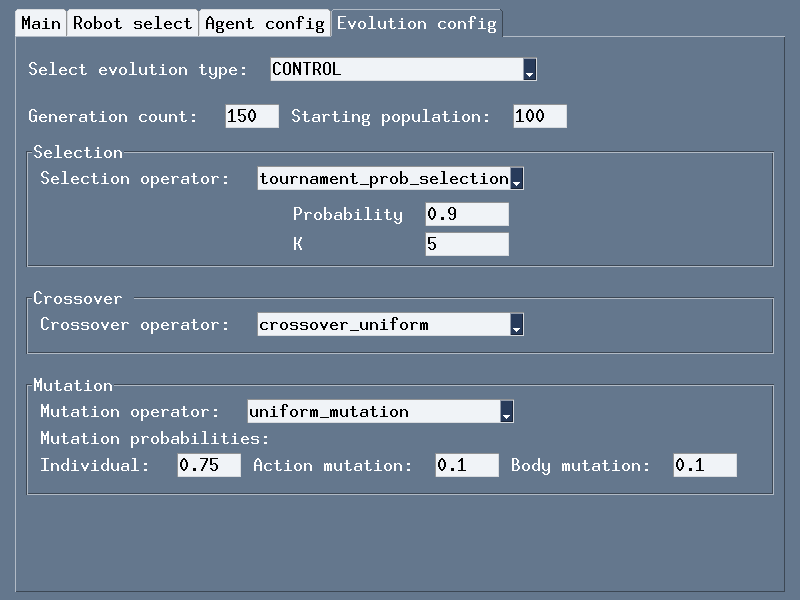
\includegraphics[width=0.6\textwidth]{../img/GUI_evo_tab.jpg}
    \caption{Okno pro úpravu specifických nastavení agenta}
    \label{imp:fig:GUI_evo}
\end{figure}


Vytváření jednotlivých sekcí je oddělené do vlastních funkcí, které jsou pak
při inicializaci aplikace volány z rozložení hlavního okna.

Běh aplikace je tak, jak tomu u grafických aplikací bývá, zajištěn nekonečným
cyklem, který se opakuje vždy při příchodu nějaké události do aplikace (např.
kliknutí myší na tlačítko v okně). Modul \emph{PySimpleGUI} pracuje na základě
posílání zpráv o událostech. Tyto zprávy jsou po obdržení zpracovávány uvnitř
nekonečného cyklu a dle potřeby vyřešeny.

Určité sekce využívají napojení na pomocné moduly z centrálního modulu
\emph{RoboEvo} (popsané výše v sekci \ref{imp:roboevo}). Tohoto využíváme
hlavně, abychom umožnili rozsáhlejší modifikace jednotlivých pomocných modulů
(např. popis a nastavování parametrů agenta).

Pokud uživatel spustí vybraný experiment, proběhne proces, ve kterém se
z~navolených hodnot v aplikaci vytvoří parametry pro spuštění experimentu
(objekt třídy \texttt{ExperimentParams}), které následně předá modulu
\emph{RoboEvo}. Zároveň se vytvoří nové okno, které vykresluje graf a vypisuje
informace o právě běžícím experimentu. Z tohoto okna může uživatel v libovolném
okamžiku zažádat o~prezentaci jedince s dosud nejlepším řešením.

\section{Textové rozhraní} \label{imp:TUI}
Vedle grafického rozhraní lze knihovnu ovládat i pomocí zadávání příkazů do
příkazové řádky. Tento přístup ke knihovně se může hodit při vypracování
větších nebo vícero experimentů, kdy očekáváme, že experimenty poběží delší
dobu (několik hodin). Pro tento účel nepotřebujeme a ani by nebylo
nejvýhodnější po celou dobu sledovat okno grafické aplikace.

Textové rozhraní (TUI) je tedy vytvořené hlavně za účelem spouštění
experimentů. Proto toto rozhraní úzce spolupracuje se třídou experimentů
(popsanou výše v sekci \ref{imp:experimentsetter}). Rozhraní vytváří jednoduchý
způsob, jak vybírat a spouštět vyhodnocení dostupných experimentů.

\paragraph{Ovládání TUI}
Textové rozhraní ovládá uživatel z příkazové řádky s různými vstupními
argumenty. Těmito argumenty jsou následující:

\begin{itemize}
    \item \texttt{-{}-experiment} -- argument, který obdrží textový vstup
        specifikující jméno jednoho nebo více experimentu (oddělených mezerou),
        jehož parametry chceme načíst a spustit (pracující s modulem
        \emph{experiment\_setter} popsaného v oddíle
        \ref{imp:experimentsetter}),
    \item \texttt{-{}-experiment\_names} -- při uvedení tohoto argumentu
        program vypíše názvy všech vytvořených experimentů z modulu
        \emph{experiment\_setter} a následně se ukončí,
    \item \texttt{-{}-batch} -- argument číselné hodnoty, specifikující
        kolikrát se má nakonfigurovaný experiment opakovaně spustit (používané
        pro statistické vyhodnocení výsledků experimentů),
    \item \texttt{-{}-batch\_note} -- textový argument umožňující připojit
        vlastní poznámku k~názvu složky, do které se experimenty z
        několikanásobného spuštění ukládají (argument nemá žádný efekt pro
        experimenty z modulu \\\emph{experiment\_setter}),
    \item \texttt{-{}-open} -- textový argument, který obdrží cestu k uloženým
        datům nejlepšího jedince z libovolného předchozího experimentu,
        umožňující vizualizaci řešení daného jedince,
    \item \texttt{-{}-no\_graph} -- argument, který značí, že za běhu algoritmu
        nemá být vykreslován graf průběhu fitness hodnot v jednotlivých
        generacích.
\end{itemize}

\paragraph{Ukázky možných vstupů}
Textové rozhraní úzce spolupracuje s modulem \emph{experiment\_setter}, který
udržuje definované experimenty. Jedním z užitečných parametrů je
\texttt{-{}-experiment\_names}, který TUI nechá vypsat názvy všech definovaných
experimentů.

\begin{code}
>>> TUI.py --experiment_names
<<< List of created experiments:
     - exp10_TFS
     - exp11_TFS_spot
     - exp12_TFS_ant
     ...
\end{code}

Pokud již známe jeden nebo více experimentů, které chceme spustit,
můžeme je spustit výběrem parametru \texttt{-{}-experiment} a vypsáním seznamu 
zvolených experimentů oddělených mezerou.

\begin{code}
>>> TUI.py --experiment exp11_TFS_spot exp_12_TFS_ant
<<< Starting experiment - exp11_TFS_spot 
    ...
\end{code}

Ve spojení s parametrem \texttt{-{}-experiment} můžeme vybrat další parametry.
Těmi mohou být parametr \texttt{-{}-batch} (\texttt{-{}-batch 5} bude
opakovat běh všech zvolených experimentů 5krát), nebo parametr
\texttt{-{}-no\_graph}, který zabrání průběžnému vykreslování grafů z běhu
experimentu nebo parametr \texttt{-{}-note}, umožňující upravit název složky,
do které se budou data ukládat.

\paragraph{}
Posledním často používaným parametrem je \texttt{-{}-open}, pomocí kterého
si můžeme v simulačním prostředí přehrát běh nejlepšího jedince ze zvoleného
předchozího experimentu.
\begin{code}
>>> TUI.py --open saved_files/runs/run1/individual.save
<<< (Simulace zvoleného jedince)
\end{code}

\paragraph{Implementace TUI}
Samotná implementace rozhraní je již velmi jednoduchá. Zpracovává uživatelské
vstupy z argumentů, které buď předává dál do korespondujících funkcí, nebo
hlásí a řeší problémy, které mohli při zadávání argumentů nastat.

%%% Fiktivní kapitola s instrukcemi k PDF/A

\chapter{Experimenty a výsledky}

\section{Vývoj řížení robotů}

\section{Vývoj řízení a morfologie robotů}

\section{Diskuze výsledků}


\chapter*{Závěr}
Práce představuje platformu pro tvorbu a provádění experimentů s evolučními
algoritmy na simulovaných robotech. Práce splnila cíle, které pro ni byly
stanoveny. Vytvořili jsme systém přístupný uživatelům s různými úrovněmi
pochopení problematiky evolučních algoritmů a zpřístupnili tak nástroj, pomocí
kterého budou uživatelé moci jednoduše prohlubovat a aplikovat své znalosti.
Platforma nabízí řadu implementovaných operátorů evolučních algoritmů a několik
robotů různých úrovní složitosti, se kterými může uživatel okamžitě pracovat.

Při tvorbě platformy jsme dbali na to, aby zdrojový kód byl srozumitelný
a~jednotlivé části logicky rozdělené, což uživatelům umožní a zjednoduší
přístup ke zdrojovému kódu. Tím nabízíme možnost hlubšího pochopení fungování
evolučních algoritmů a jejich případného rozšiřování a aplikování nových
vlastních částí.

Experimenty provedené v této práci ukazují jak typy experimentů,
které~platforma umožňuje, tak styly jejich vyhodnocení. Pomocí experimentů jsme
na dvou robotech různých složitostí ověřili fakt, že jednoduché evoluční
algoritmy nestačí pro řešení všech problémů, a že pro určité pokročilé problémy
je třeba pokročilých evolučních algoritmů. 

Zároveň jsme demonstrovali příklady experimentů, které umožňují vývoj jak
řízení, tak morfologie robotů. Pro tento problém jsme v práci navrhli a
implementovali způsob, jakým je možné za běhu algoritmů měnit XML konfigurační
soubory robotů z knihovny \emph{MuJoCo}. Tyto experimenty předvedly zajímavé
výsledky, vytvářející roboty různých konfigurací, které byly schopné dosáhnout
lepších výsledků než ty výchozí.

Práce nabízí mnoho možností pro rozšiřování. Vedle pokročilejších evolučních
algoritmů na vývoj řízení robotů by zajímavým rozšířením mohlo být prozkoumání dalších
možností vývoje morfologie, umožňující rozsáhlejší změny v konfiguraci robotů.
Dalším by mohlo být podrobnější zkoumání dopadů různých fitness funkcí na
výsledky evolučního vývoje.

\addcontentsline{toc}{chapter}{Závěr}


%%% Seznam použité literatury
%%% Seznam použité literatury (bibliografie)
%%%
%%% Pro vytváření bibliografie používáme bibTeX. Ten zpracovává
%%% citace v textu (např. makro \cite{...}) a vyhledává k nim literaturu
%%% v souboru literatura.bib.
%%%
%%% Příkaz \bibliographystyle určuje, jakým stylem budou citovány odkazy
%%% v textu. V závorce je název zvoleného souboru .bst. Styly plainnat
%%% a unsrt jsou standardní součástí latexových distribucí. Styl czplainnat
%%% je dodáván s touto šablonou a bibTeX ho hledá v aktuálním adresáři.

\bibliographystyle{czplainnat}    %% Autor (rok) s českými spojkami
% \bibliographystyle{plainnat}    %% Autor (rok) s anglickými spojkami
% \bibliographystyle{unsrt}       %% [číslo]

\renewcommand{\bibname}{Seznam použité literatury}

%%% Vytvoření seznamu literatury. Pozor, pokud jste necitovali ani jednu
%%% položku, seznam se automaticky vynechá.

\bibliography{literatura}

%%% Kdybyste chtěli bibliografii vytvářet ručně (bez bibTeXu), lze to udělat
%%% následovně. V takovém případě se řiďte normou ISO 690 a zvyklostmi v oboru.

% \begin{thebibliography}{99}
%
% \bibitem{lamport94}
%   {\sc Lamport,} Leslie.
%   \emph{\LaTeX: A Document Preparation System}.
%   2. vydání.
%   Massachusetts: Addison Wesley, 1994.
%   ISBN 0-201-52983-1.
%
% \end{thebibliography}


%%% Obrázky v bakalářské práci
%%% (pokud jich je malé množství, obvykle není třeba seznam uvádět)

% \listoffigures

%%% Tabulky v bakalářské práci (opět nemusí být nutné uvádět)
%%% U matematických prací může být lepší přemístit seznam tabulek na začátek práce.

% \listoftables

%%% Použité zkratky v bakalářské práci (opět nemusí být nutné uvádět)
%%% U matematických prací může být lepší přemístit seznam zkratek na začátek práce.
% \chapwithtoc{Seznam použitých zkratek}

%%% Přílohy k bakalářské práci, existují-li. Každá příloha musí být alespoň jednou
%%% odkazována z vlastního textu práce. Přílohy se číslují.
%%%
%%% Do tištěné verze se spíše hodí přílohy, které lze číst a prohlížet (dodatečné
%%% tabulky a grafy, různé textové doplňky, ukázky výstupů z počítačových programů,
%%% apod.). Do elektronické verze se hodí přílohy, které budou spíše používány
%%% v elektronické podobě než čteny (zdrojové kódy programů, datové soubory,
%%% interaktivní grafy apod.). Elektronické přílohy se nahrávají do SISu a lze
%%% je také do práce vložit na CD/DVD. Povolené formáty souborů specifikuje
%%% opatření rektora č. 72/2017.
\appendix
\chapter{Přílohy}

\section{První příloha}

\openright
\end{document}
